\documentclass[paper=a4, fontsize=11pt, openany]{book}
% https://stackoverflow.com/questions/491904/how-do-i-remove-blank-pages-coming-between-two-chapters-in-appendix
\usepackage[top=1.8cm, bottom=2.54cm, left=2.25cm, right=2.25cm]{geometry}
\usepackage[utf8]{inputenc}
\usepackage{graphicx} % use includegraphics to import jpegs --- FIXME... see below
\usepackage[british]{babel} % English language/hyphenation
\usepackage{pdfcomment}
\usepackage{amsmath,amsfonts,amsthm} % Math packages
\usepackage{lipsum} % Used for inserting dummy 'Lorem ipsum' text into the template
\usepackage{sectsty} % Allows customizing section commands
\usepackage{color}
\usepackage{parskip}
\usepackage[usenames,dvipsnames,svgnames,table]{xcolor}
%\usepackage[]{nohyperref}  % This makes hyperref commands do nothing without errors
\usepackage{url}  % This makes \url work
% http://tex.stackexchange.com/questions/667/typeset-url-in-a-non-typewriter-font
\urlstyle{same}
% allow manual caption/figure numbering
% http://tex.stackexchange.com/questions/199207/no-caption-number-for-figures-and-tables
\usepackage{caption}
\usepackage{multicol}

\hypersetup{hidelinks}


\usepackage{fourier} % Use the Adobe N-Utopia font for the document - comment this line to return to the LaTeX default

\usepackage{fancyhdr} % Custom headers and footers
\pagestyle{fancyplain} % Makes all pages in the document conform to the custom headers and footers
\fancyhead{} % No page header - if you want one, create it in the same way as the footers below
\fancyfoot[L]{} % Empty left footer
\fancyfoot[C]{} % Empty center footer
\fancyfoot[R]{\thepage} % Page numbering for right footer
\renewcommand{\headrulewidth}{0pt} % Remove header underlines
\renewcommand{\footrulewidth}{0pt} % Remove footer underlines
\setlength{\headheight}{13.6pt} % Customize the height of the header
\numberwithin{equation}{section} % Number equations within sections (i.e. 1.1, 1.2, 2.1, 2.2 instead of 1, 2, 3, 4)
%\numberwithin{figure}{section} % Number figures within sections (i.e. 1.1, 1.2, 2.1, 2.2 instead of 1, 2, 3, 4)
\numberwithin{table}{section} % Number tables within sections (i.e. 1.1, 1.2, 2.1, 2.2 instead of 1, 2, 3, 4)
\setlength\parindent{0pt} % Removes all indentation from paragraphs - comment this line for an assignment with lots of text

% https://www.sharelatex.com/learn/Typesetting_quotations
\usepackage{epigraph}
% \epigraph{All human things are subject to decay, and when fate summons, Monarchs must obey}{\textit{Mac Flecknoe \\ John Dryden}}

\title{Drucksache 1}

\date{2. Auflage, aktualisiert. Jetzt noch deprimierender. Smiley!}

% Mail/Link author?
\author{Claudia Latour / Martin Sonneborn \\
 \textbf{Assange}
}

% allow multi-line comments using \begin{comment} ... \end{comment}
\usepackage{verbatim}



\begin{document}

%% https://tex.stackexchange.com/questions/351540/having-chapters-shown-as-numbers-and-roman-letters
\renewcommand{\thechapter}{\Roman{chapter}}

\maketitle % Print the title

\chapter*{Preface}

Dreamworks und Universal sind an einem konzisen Manuskript zum
Leben von Julian Assange gescheitert, genauso wie die New York Times
und der Guardian.
Wir auch.
Nehmen Sie, was jetzt dabei herausgekommen ist, als Plädoyer für Demokratie \& Bürgerrechte (am Beispiel eines Publizisten und Plattformgründers), für eine freie Gesellschaft, freie Presse und freie Information.
Oder als Sympathieerklärung an das Projekt von WikiLeaks - und Antipathieerklärung an all jene, die es bekämpfen.

%% FIXME: FUSS !

Herausgeber:
Martin Sonneborn
Fraktionsloses Mitglied des Europäischen Parlaments
Rue Wiertz 60
1047 Brüssel
Belgien
2. Auflage, aktualisiert. Jetzt noch deprimierender. Smiley!
Die zum Ausdruck gebrachten Meinungen liegen in der alleinigen Verantwortung der jeweiligen Verfasser
und geben nicht unbedingt den offiziellen Standpunkt des Europäischen Parlaments wieder.

\tableofcontents

%% START 2-column layout == Zweispaltiges Layout. Am ENDE DES DOKUMENTS erfolgt \end...
\begin{multicols}{2}

%% TODO: This should print above chapter 1, not below table of contents.
\epigraph{„Das Politische kann, wo Menschen leben, nicht verschwinden.“}{\textit{J. Habermas}}


%%%%%%%%%%%%%%%%%%%%%%%%%%%%%%%%%%%%%%%%%%%%%%%%%%%%%%%%%%%%%%%%%%%%%%%%%%%%%%%

\chapter{Mehr Sein als Schein}
Es gehört zu den Erkenntnissen, die einem in Jurisprudenz und Jurisdiktion ungeschulten Beobachter nicht
neu sein dürften, dass die WIRKLICHKEIT eines juristischen VERFAHRENS manchmal nur noch wenig mit der
WIRKLICHKEIT des ihm zugrundeliegenden (RECHTS)
FALLES zu tun hat. Erst recht nicht mit dem DIESEM
wiederum zugrundeliegenden SACHVERHALT. Und am
wenigsten mit der gesellschaftspolitischen und demokratiepraktischen REALITÄT, die sich in ALL DEM konzentriert.
Wenn die WIRKLICHKEIT einer GERICHTLICHEN VERHANDLUNG sich von ihrer übergeordneten BEDEUTUNG, von ihren Auslösern, Gründen, Ursachen, Absichten, Zielen \& Folgen - und damit von dem im Grunde
verhandelnswerten POLITISCHEN KERN - vollends
LOSGELÖST hat, um in der absurden SCHEINREALITÄT eines von juristischen Scheinpflöcken eingehegten
Scheingeländes (in unaufhaltsamem Wahnsinn) vor sich
hinzutreiben, dann befindet man sich im Berufungsverfahren um die Auslieferung des WikiLeaks-Gründers
Julian Assange.
Womöglich wurden die seit Jahrhunderten durch nichts
als ihr schieres Vorhandensein beglaubigten Prozeduren und Praxen unserer JUSTIZSYSTEME am Ende nun
doch von diesen (selbst)zerstörerischen Ausläufern der
Spätmoderne ereilt - und zwar jeder ihrer noch so aufdringlich zur Schau gestellten HISTORIZITÄTEN zum
Trotz. Das gilt natürlich umso mehr für Großbritanniens
Magna Carta und ihre echtholzvertäfelten Wände, viktorianischen Samtvorhänge, smaragdgrünen Bankierlampen (Art Déco) und (gut gepuderten) Richterperücken.
Vor der plakativen Kulisse derartiger „Rechtstraditionen“
sind im gesellschaftlichen Subsystem der Rechtspflege
längst DENKFIGUREN und ARGUMENTATIONSMUSTER entstanden, die (in sonderbarer Selbstreferentialität und blödsinnigster Binnensymbolik) so stur um ihr
EIGENTÜMLICHES EIGENLEBEN kreisen, dass sie mit
gesellschaftlich relevanten Fragen, Zuständen und Implikationen tatsächlich nicht mehr im Entferntesten verbunden sind.


%%%%%%%%%%%%%%%%%%%%%%%%%%%%%%%%%%%%%%%%%%%%%%%%%%%%%%%%%%%%%%%%%%%%%%%%%%%%%%%

\chapter{„Ja, warum nicht?“}
Am 27. und 28. Oktober 2021 wohnen wir in London
einer Verhandlung bei, in der das EIGENTLICH VERHANDELNSWERTE, das ja NIEMALS nur Julian Assange selbst, sondern immer UNS ALLE betroffen hat, erst
1

2

gar nicht AUSGESPROCHEN wird. Die (seit 1066) minutiös eingeübten Verfahrensregeln wollen es so. Dass hier
nämlich nicht das große Ganze SELBST, sondern nur seine rechtsterminologisch zulässigen WRITS zur Verhandlung stehen. Mit denen nicht das große Ganze SELBST,
sondern nur die von DIESER besonderen BERUFUNG
betroffenen TEILE (s)einer auf juristischem Wege erzeugten „Wirklichkeit“ erfasst werden.
Und so kommt es tatsächlich, dass an vollen zwei Verhandlungstagen am höchsten britischen Gericht, dem
Londoner High Court, die im Fall Assange konzentrierte HAUPTFRAGE gar nicht erst auftaucht. Die natürlich
noch immer darin besteht, ob ein angeblich demokratischer Rechtsstaat ein über 100 Jahre altes US-amerikanisches (Anti-)Spionagegesetz zweckentfremden darf,
um - assistiert von traditionsgesättigten Justizapparaten
befreundeter Rechtsstaaten (der alteuropäischen Welt) in einer tausendjährigen Verfolgungsjagd beispiellosen
Ausmaßes einen australischen Publizisten so gründlich
zu vernichten, dass allein das an ihm statuierte Exempel - seiner entfalteten ABSCHRECKUNGSWIRKUNG
wegen - jeglichen Investigativjournalismus einer Vierten
Kraft, die diesen Namen auch nur annähernd noch verdienen will, fortan nachhaltig unterbinden wird.
Das britische Bezirksgericht, an dem der australische
Publizist Julian Assange nach einer kafkaesken Kaskade
staatsanwaltlicher (und staatlicher) Manöver im vergangenen Jahr schlussendlich gestrandet war, hatte diese
Frage im Januar d.J. verstörenderweise mit „JA, WARUM
NICHT?“ beantwortet, was den größten demokratischen
SKANDAL in der Geschichte der Demokratie hätte auslösen müssen.
Geführt worden war das erstinstanzliche Verfahren (etwas überraschend) von einer biederen Bezirksrichterin
(District Judge) namens Vanessa Baraitser, seinerzeit das
unbeschriebenste Blatt, das die britische Gerichtsbarkeit
zu bieten hatte. Öffentlich bekannt war weder ihr fachlicher Hintergrund noch ihre Vita oder eine Übersicht
der von ihr verhandelten Fälle - noch nicht mal eine verwackelte Photographie. Die durchschnittliche Besitzerin
einer ländlichen Autowaschanlage habe im Netz mehr
Beweise für ihre tatsächliche Existenz hinterlassen als
Vanessa Baraitser, bemerkte der britische Ex-Diplomat
Craig Murray.1
Eine Handvoll Bagatellverfahren waren ihr wohl zugeteilt worden, immerhin aufregend genug für die traditionell aufregungsbereite (britische) Lokalpresse: Sexuelle
Belästigungen von und mit Polizisten, Provinzpolitiker
mit einem Faible für heimliche Handyschnappschnüsse unter vorüberschreitenden Rockträgerinnen, solche
Sachen. In zehn Jahren Bezirksgerichtspraxis hatte Baraitser ein einziges Auslieferungsverfahren verhandelt:

Craig Murray über Baraitser: „Jemand schlug mir vor, sie könnte ein Hologramm sein, aber ich denke nicht. Hologramme haben mehr Einfühlungsvermögen.“

Frankreichs Ersuchen nach Überstellung eines in staatliche Korruption um Ex-Präsident Nicolas Sarkozy verwickelten Geschäftsmannes (Alexandre Djouhri). Die
Sache war klar, Baraitser hatte sie zustimmend beschieden.
Und nun also der Fall Assange.

%%%%%%%%%%%%%%%%%%%%%%%%%%%%%%%%%%%%%%%%%%%%%%%%%%%%%%%%%%%%%%%%%%%%%%%%%%%%%%%

\chapter{Echt krimineller Shit} % III.
Bevor irgendjemand sich irgendein Urteil über Julian
Assange bildet, sollte er sich noch einmal in Erinnerung
rufen, mit wem (und mit was) er es da eigentlich zu tun
hat.
Fleißige Statistiker haben ausgerechnet, dass die kleine Gruppe von Aktivisten um WikiLeaks in zehn Jahren
ZEHN MILLIONEN Geheimdokumente veröffentlicht
hat. Mehr als die gesamte Weltpresse, seit es die gesamte
Weltpresse überhaupt gibt. Dokumente über Kriegsverbrechen, Menschenrechtsverletzungen, Folter, Gewalt,
Entführungen, illegale Überwachung, Spionage, Meinungsmanipulation und Umweltverbrechen.
Einschlägige Veröffentlichungen umfassen diplomatische und militärische Geheimpapiere (führender kriegführender Staaten) sowie Dokumente zur Sichtbarmachung der Vorgehensweisen gesellschaftswirksamer
Organisationen und Einzelakteure - (verlogene) Regierungen, (machtbesessene) Parteiapparate, (korrupte)
Politiker, (unsympathische) Unternehmer, (Arschloch-)
Konzerne und (notorische) Egomanen, (Schweizer)
Banken, (Offshore-)Betrüger, (profitfixierte) Naturzerstörer und schließlich politische („Hillary“) und religiöse
(„Scientology“) Sekten. WikiLeaks-Publikationen waren
dabei nie Selbstzweck, sondern Mittel zur Erreichung
eines zutiefst demokratischen Ziels, das - getragen von
einem ganz schön altmodischen Menschheits- und Gesellschaftsideal2 - auf die (unumstößliche) Überzeugung
zurückgeht, dass eine FREIE GESELLSCHAFT nur auf
FREIER INFORMATION gegründet sein kann.
Im Projekt von WikiLeaks verdichtet sich die grundlegende Frage moderner Demokratien, nämlich die nach
der LEGITIMIERBARKEIT von staatlichen, nachrichtendienstlichen und militärischen Informationsmonopolen.
WikiLeaks stellt Fragen, die jeder mündige Bürger3 sich
und seinen demokratischen Repräsentanten (und -onkeln) stellen sollte: Hat eine Regierung das Recht, sich
(mit dem Ziel des Machterhalts oder der Bereicherung)
über geltendes Recht hinwegzusetzen? Hat ein Nachrichtendienst das Recht, die Persönlichkeitsrechte von
Bürgern zu verletzen, zu deren Schutz er bestellt ist?
Hat ein Militär das Recht, gegen Menschenrechte oder
2
3

Prinzipien des Völkerrechts zu verstoßen? Und, falls ja,
haben diese Organisationen zudem noch das Recht, ihre
Rechtsverstöße durch Geheimhaltung vor der Öffentlichkeit zu verbergen?
Assange, ein mehrfach preisgekrönter Journalist und
Verleger, wird seit April 2019 rechtsgrundlos im britischen Hochsicherheitsgefängnis Belmarsh festgehalten
- zusammen mit Terroristen und Schwerverbrechern,
Serienmördern, Sexualstraftätern, Islamisten, Rechtsextremisten, IRA-Kämpfern und Christoph Waltz, der
als Ernst Stavro Blofeld von hier aus zuletzt sein bionisches Auge einsetzte, um den (fehlschlagenden) Befehl
zur Tötung von James Bond zu geben. Belmarsh ist das
britische Guantanamo, eine streng geometrische Zuchtanstalt mit klinisch weißen Innenzellen, ein Ort, der den
(treffenden) Spitznamen HELLMARSH trägt. Hier sitzt
der WikiLeaks-Gründer seit 30 Monaten in Einzelhaft trotz wiederholter Erklärungen der Vereinten Nationen
(und anderer), wonach er Opfer willkürlicher, illegaler Inhaftierung und psychologischer Folter ist. Es gibt,
das muss man sich immer wieder klar machen, KEINE
RECHTSGRUNDLAGE für die Inhaftierung von Julian
Assange. In Großbritannien liegt nicht das Geringste
gegen ihn vor.
Sachdienlicher Hinweis von Ross Kemp
Nachdem wir Teile der Dokumentation „Welcome to
HMP Belmarsh“ gesehen haben, für die der Schauspieler
Ross Kemp („EastEnders“) erstmals Drehgenehmigung
und Zugang zum Hochsicherheitsgefängnis erhalten hatte, sind wir fast ein bisschen erleichtert, dass Assange dort
wenigstens in einem Einzelzimmer untergebracht ist.
Und wir sind entsetzt, wirklich fassungslos, dass man ihn
seiner Freiheit beraubt, um ihn ohne Rechtsgrundlage an
einen solchen Ort zu zwingen. Ross Kemp ist ein Mann wie
ein Wohnzimmerschrank und ziemlich hart im Nehmen.
Weltweit hat er schon unter kriminellen Straßengangs, in
Afghanistan, Papua-Neuguinea und werweißwonoch als
„embedded journalist“ gedreht, ohne mit einer einzigen
Wimper zu zucken. Als er „The Box“, die Hochsicherheitseinheit des Gefängnisses, betritt und sich nur kurz die
Tür hinter ihm schließt, ist er am bedrückendsten Ort der
ganzen Welt, sagt er. Es gibt kein Bett, kein Waschbecken,
keine Toilette, kein Fenster, keinen Zugang zu Wasser oder
zu Luft. „Man spürt, dass man völlig allein ist. Ich glaube
nicht, dass ich eine Stunde hier drin verbringen könnte,
ohne wahnsinnig zu werden.“
Im erstinstanzlichen Verfahren um seine Auslieferung
hatte Bezirksrichterin Baraitser sich verbissen geweigert,
jeden der auf der Hand liegenden Sachverhalte auch nur
zur Kenntnis zu nehmen - vom genuin JOURNALISTISCHEN Charakter der Veröffentlichungen von WikiLeaks
über die erkennbar POLITISCHE Natur der gegen seinen
Gründer gerichteten Anwürfe bis hin zur (wirklich auch

Aufklärung!
Im Sinne Kants, Voltaires, Daisy Ducks \& R.D. Prechts

3

für Blinde) offensichtlichen Aussicht auf ein unfaires Gerichtsverfahren in den USA.
Assange würde in ALEXANDRIA im US-Bundesstaat Virginia vor Gericht gestellt werden, wo er sich einem geheimen Verfahren vor einem Sondergericht mit Grand
Jury stellen müsste. In unmittelbarster Nähe dieser
Stadt, in Washington und Langley, befinden sich das
Pentagon, die Defense Intelligence Agency, das FBI, die
CIA, die NSA sowie die Hauptquartiere weiterer Militär-,
Sicherheits- und Geheimdiensteinrichtungen der USA.
Die Einwohnerstruktur von Alexandria ist von einer
durchschnittlichen Stadtbevölkerung in etwa so weit
entfernt wie dieser lächerliche Prozess hier von einem
rechtsstaatlichen Verfahren. Zwischen 80 und 90 Prozent
der volljährigen Bewohner Alexandrias, unter denen die
Laienrichter im Verfahren gegen Assange rekrutiert würden, sind Vertreter von Regierungsbehörden, Geheimdiensten oder des US-Militärs und stehen in einem direkten, indirekten oder (wenigstens) wirtschaftlichen
Abhängigkeitsverhältnis zur US-Regierung. Grand Jurys
im zuständigen Gerichtsbezirk sind so zuverlässig einäugig, einohrig, einseitig, parteiisch und voreingenommen, dass man eine objektive Urteilsfindung von ihnen nicht ernsthaft erwarten kann - die Loyalitätslast
gegenüber der Regierung ist erdrückend. In der langen
Geschichte des Eastern District Court of Virginia gab es
noch nie auch nur einen einzigen Fall, in dem die Grand
Jury einen von den nationalen Sicherheitsbehörden Angeklagten freigesprochen hätte. Wirklich noch nie.
Sachdienlicher Hinweis von heise.de
US-amerikanische Rechtsvereinigungen wie die American Association of Jurists (AAJ) und das Center for Constitutional Rights (CCR) haben gemeinsam mit international arbeitenden juristischen Institutionen und Juristen
einen Brief an den britischen Premierminister Boris Johnson und seine Regierung geschrieben, um ihn von einer
Auslieferung Julian Assanges an die USA abzuhalten. Ein
solcher Schritt wäre ihrer Ansicht nach illegal:
„Die Auslieferung wäre rechtswidrig, da der Schutz der
grundlegenden Prozessrechte von Herrn Assange in den
USA nicht gewährleistet ist. Herr Assange wird vor dem
berüchtigten „Spionagegericht“ des Eastern District of
Virginia (in Alexandria, die Verf.) vor Gericht gestellt, vor
dem kein Angeklagter der nationalen Sicherheit jemals
Erfolg hatte. Hier sieht er sich einem geheimen Verfahren vor einer Jury ausgesetzt, die aus einer Bevölkerung
ausgewählt wurde, in der die meisten Personen, die für
die Auswahl der Jury in Frage kommen, für die CIA, NSA,
DOD oder DOS (The Central Intelligence Agency, The National Security Agency, U.S. Department of Defense, U.S.
Department of State) arbeiten oder mit dieser verbunden
sind.“

4

4

(Aua, aua.)

%%%%%%%%%%%%%%%%%%%%%%%%%%%%%%%%%%%%%%%%%%%%%%%%%%%%%%%%%%%%%%%%%%%%%%%%%%%%%%%

\chapter{„Raaache!“ (Fatty Pompeo)}
Den Vereinigten Staaten von Amerika war Assange nach
der Veröffentlichung der (vom US-Militär penibel unter
Verschluss gehaltenen) Materialien zu den Kriegen im
IRAK und in AFGHANISTAN spätestens mit den Publikationen zu Menschenrechtsverletzungen im Gefangenenlager Guantanamo Bay verbindlich auf die Zehen
getreten.4
Unter Barack OBAMA hatten die USA noch auf eine
Anklage gegen Assange verzichtet - nicht aus Menschenfreundlichkeit, sondern eines handfesten Definitionsdilemmas wegen, das unter Juristen als das
„New-York-Times-Problem“ bekannt ist. Es geht ungefähr so: Wie kann man Julian Assange wegen der Veröffentlichung von als geheim eingestuftem Material (auf
den Seiten von WikiLeaks) verfolgen - NICHT ABER die
Chefredakteure der New York Times, auf deren Seiten
doch GENAU DASSELBE stand? Oder die Herausgeber
von The Guardian, Le Monde, El Pais, Corriere della Sera,
Süddeutsche Zeitung oder Der Spiegel?
Damit hier nicht (aus Versehen) ein falscher Eindruck
entsteht: Unter der Regierung Obama sind die US-amerikanischen Geheimdienste und Justizbehörden natürlich ebenfalls gegen Assange vorgegangen. 2011 hat das
FBI eine großangelegte Infiltrationsoperation gegen WikiLeaks in Island durchgeführt, einen Pädophilen als falschen Zeugen angeworben und - in Vorbereitung einer
Anklage - bereits die passende Grand Jury einberufen.
Vorläufig zurückgestellt wurde lediglich die Einleitung
eines Verfahrens, und dies nur auf dringendes Anraten
von Rechtsanwälten, denen (im Weißen Haus) schlagartig der Inhalt des „First Amendment“ eingefallen war.
Den feinsinnigen Rechtsphilosophen um Donald
TRUMP ging diese Sache mit der fehlenden Trennschärfe (zwischen Publizisten und Publizisten) freilich am
Arsch vorbei.
2017 hatte WikiLeaks die (beunruhigenden) Fähigkeiten
des amerikanischen Geheimdienstes zu elektronischer
Überwachung und Cyber-Kriegsführung öffentlich gemacht. Das sogenannte „Vault 7“-Leak war das „größte“ und - der New York Times zufolge - wirklich auch
das „peinlichste“ Datenleck, das der CIA je passiert war
- oder einem ihrer Behördenleiter. Für den damaligen
CIA-Chef (und späteren Außenminister) Mike Pompeo
mag es (darüber hinaus) eine (narzisstische) Kränkung
gewesen sein (oder nicht). Jedenfalls war es der Auslöser
für eine seither mit allen nur denkbaren Mitteln geführte
(Privat-)Vendetta gegen WikiLeaks und Julian Assange.
Fatty Pompeo wollte RACHE. Und erklärte WikiLeaks offiziell zum „feindlichen nichtstaatlichen Geheimdienst“
- eine seinem Erfinder an plumper Bösartigkeit in nichts

nachstehende Begriffsneuschöpfung, von der kein seriöser Staatsrechtler zuvor (oder seitdem) jemals gehört
hat.5
Mit Trump und Pompeo im Rücken erhob das US-Justizdepartment schließlich seine waghalsige Anklage gegen
Julian Assange. Die Schrift umfasst 18 Punkte (das sind
mehr als ein westeuropäischer Marienkäfer hat) und
stellt ihm nach Auslieferung eine Haftstrafe von 175 Jahren in Aussicht - je zehn Jahre für jeden der 17 Anklagepunkte unter dem Espionage Act und weitere fünf für
den 18., in dem ihm das versuchte Eindringen in einen
Regierungscomputer unterstellt wird, ein Verstoß nach
dem „Computer Fraud and Abuse Act“.
Noch einmal zur Erinnerung: KEIN EINZIGER der USamerikanischen Kriegsverbrecher, die im Irak, Afghanistan oder Guantanamo erwiesenermaßen ihr Unwesen
getrieben, Unschuldige, Zivilisten, Kinder gequält, gefoltert und ermordet hatten, wurde für sein Verbrechen
je zur Rechenschaft gezogen, angeklagt oder vor Gericht
gestellt. Sie alle sind auf freiem Fuß. Zur Rechenschaft
gezogen, angeklagt und vor Gericht gestellt werden soll
hier der, der ihre Verbrechen öffentlich gemacht hat.
Die Vereinigten Staaten stützen sich dabei im wesentlichen auf den Espionage Act, ein Gesetz aus dem Jahr
1917, das unter Weltkriegsbedingungen für Weltkriegsgeheimnisträger und Weltkriegsinformationen von weltkriegsmilitärischer Sensibilität entwickelt wurde - wo
hat die Division General Custer ihre Haubitzen geparkt?
Allein diese in Ermangelung eines plausiblen, justiziablen (oder sonstwie stichhaltigen) Tatvorwurfs hervorgekramte „Rechtsgrundlage“ müsste jedem der PRÄMODERNE geistig entwachsenen Europäer (gründlich) zu
denken geben. Der Versuch, ein überholtes Kriegsgesetz
über 100 Jahre später völlig kontextenthoben gegen einen ausländischen Publizisten zur Anwendung zu bringen6, entspricht der putzigen Idee des Irren vom Bosporus, eine zeitgenössische Satire von Jan Böhmermann
mit dem reichsdeutschen Majestätsbeleidigungsgesetz
(anno 1871) zur Strecke zu bringen. Beides ist schon
auf den allerersten Blick so abwegig, dass es keines umständlicheren Kommentars dazu bedarf. Wir halten fest:
Es gibt keine Rechtsgrundlage, um einen australischen
Journalisten nach dem US-Spionagegesetz vor Gericht
zu stellen.
Die US-Anklage ist nicht nur völlig aus der Zeit gefallen
und absolut absurd, sie ist auch wirklich verfassungs-

widrig, denn sie kriminalisiert die journalistische Kernaktivität und hebt damit jahrhundertealte Rechtsgrundsätze auf, allen voran das der Rede- und natürlich das
der Pressefreiheit.

%%%%%%%%%%%%%%%%%%%%%%%%%%%%%%%%%%%%%%%%%%%%%%%%%%%%%%%%%%%%%%%%%%%%%%%%%%%%%%%

\chapter{Ping, Pong \& Psychologie} % V. = 5
Dennoch hatte Bezirksrichterin Baraitser nach mehrwöchiger Verhandlung die irrwitzige Auffassung vertreten, der Auslieferung Assanges stünde nicht die OFFENSICHTLICHE UNGEHEUERLICHKEIT einer mit
protojuristischen Winkelzügen konstruierten Anklageschrift entgegen, sondern lediglich - Tätärääää! - die
nach sieben Jahren Isolation in der Ecuadorianischen
Botschaft und weiteren zweieinhalb Jahren rechtsgrundloser Inhaftierung (ziemlich überraschungsfrei)
in Mitleidenschaft geratene psychische Verfassung des
zu Unrecht festgehaltenen Häftlings. Ergänzt um dessen
manifeste Suizidgefährdung, die durch die in aller Welt
bekannten US-amerikanischen Haftbedingungen samt
ihrer gewohnheitsmäßigen Bestialität vorhersehbar verstärkt würde.
Bei Assange, so Baraitsers Urteil, liege ein prekärer psychischer Zustand vor, der sich angesichts der „harten
Bedingungen“ des unmenschlichen US-Gefängnissystems verschlechtern würde, was ihn „zum Selbstmord
veranlassen“ könne. Rule, Britannia.
Dabei lässt Baraitsers Urteil die haarsträubenden
„Rechtsgründe“ der USA, die ein ECHTES FANGIRL des
britannischen Rule of Law kunstfertig in der Luft hätte
zerreißen müssen, fatalerweise völlig unangetastet - und
bestätigt, indem sie sie nicht ausdrücklich verwirft, damit implizit ihre Zulässigkeit. Das ist echt krass. Noch
krasser ist eigentlich nur, dass ihr Urteil das Verhandlungsgeschehen vom SCHLACHTFELD der PRESSEFREIHEIT, die natürlich alle Demokraten und Bürger
und Menschen der Welt betrifft, auf die Ebene einer individuellen SCHICKSALSBEURTEILUNG transponiert,
in der just nicht mehr das große Ganze einer gefährdeten Gesellschaftsordnung, sondern nur mehr die technischen und interpretativen Details medizino-psychologischer Gutachten eine Rolle spielen.
Allein das war und ist (ohne jeden Zweifel) ein rechtsstaatlicher Skandal. Und zwar ein multipler. Hugh.
Ein WEITERER kommt nun dadurch hinzu, dass das
hier (nachgelagert) geführte BERUFUNGSVERFAHREN

Die Pressekonferenz, in der Pompeo WikiLeaks diesen feierlichen Ehrentitel erklärt, wird von rückblickenden
Politikwissenschaftlern als einer der kardinalen Wendepunkte markiert werden müssen, an dem die (post-)
demokratische Ordnung der westlichen Welt ihrem dialektischen Umschlagspunkt ins Auge sah.
6
Selbstverständlich wurde es schon zu Zeiten des Ersten Weltkriegs von der US-Justiz zweckentfremdet, um Vertreter der politischen Opposition, Sozialisten oder Pazifisten zum Schweigen zu bringen. Eine Praxis, die die
USA bis in die späten Sechziger Jahre (und darüber hinaus) beibehalten sollten. Aufsehen erregte etwa der 1971
(gescheiterte) Prozess gegen die Militäranalysten Daniel Ellsberg und Anthony Russo, die der New York Times,
Washington Post u.a. Dokumente überlassen hatten, die belegen, dass die US-Regierung die Öffentlichkeit seit
Jahren über den Vietnamkrieg belogen hatte („Pentagon Papers“).
5

5

im engmaschigen Netz des von der ersten Instanz vorgegebenen Begründungsrahmens gefangen ist - und die
gerichtliche Erörterung sich nahezu vollumfänglich auf
das unerschöpflich vage (\& zudem zuverlässig persönlichkeitsverletzende) Feld der PSYCHOLOGIE begibt.
Und so kommt es tatsächlich, dass die anwaltlichen
Ausführungen im bedeutendsten Rechtsstreit zur Pressefreiheit der Gegenwart sich auf ein PING PONG aus
substanzfreien Unterstellungen, küchenpsychologischen Mutmaßungen und deren fachgemäßer Widerlegung reduzieren. VORGEBRACHT von James Lewis (in
der Rolle des PING), einem versierten Schießhund der
Krone, der hier natürlich nicht im Dienste Seiner Majestät, sondern höchst unfeiner Beschwerdeführer aus den
USA steht. Und WIDERLEGT von Edward Fitzgerald \&
Mark Summers (Team PONG), zwei mit derlei Blödsinn
sichtlich unterforderte Menschenrechtsanwälte auf Seiten der Verteidigung.
Sollte die Encyclopaedia Britannica je einen Eintrag zum
Begriff „groteske Dysfunktionalitäten archaotraditionalistischer Rechtssysteme“ planen, hätten wir da einen
Knoten im Taschentuch, den wir bestimmt nie vergessen
werden. Knoten ist im Taschentuch, Ihr Vögel. Knot is in
the handkerchief. You birds.

%%%%%%%%%%%%%%%%%%%%%%%%%%%%%%%%%%%%%%%%%%%%%%%%%%%%%%%%%%%%%%%%%%%%%%%%%%%%%%%

\chapter{Im holzvertäfelten Herzen der Macht} % 6

Das Gerichtsgebäude der Royal Courts of Justice in der
Londoner Innenstadt ist ein ehrgebietender Ort voll
säkularer Sakralität und vollholzgepflasterter Gerichtssaalminiaturen. Hier kommen - nach der letzten Reform
von 1873 (HÖRT, HÖRT!) - nicht nur die bedeutendsten
Common-Law-Gerichte einschließlich des Höchsten
und des Berufungsgerichts zusammen, sondern in einer
winzigen Trachtenstube namens COURT ROOM FOUR7
also auch besagter Anklagevertretervertreter James Lewis (Perücke: Langhaar, Ziege) sowie Edward Fitzgerald
(Langhaar, Ross) und Mark Summers (Langhaar, unecht),
die Verteidiger von Julian Assange (Langhaar, echt).
Ihre rabenschwarzen Roben reichen bis zu den Spitzen
ihres jeweiligen Schuhwerks herunter, was sich - zumindest nach ein paar Pints - als potentiell halsbrecherische Tradition entpuppen könnte. Spätestens seit der
Studentenbewegung dürfte allgemein bekannt sein, was
UNTER DEN TALAREN in aller Regel so verborgen ist,
hier ist das alles 300 Jahre alt. Seine schmutziggrauen
Flechtperücken verdankt der feine Londoner Anwaltsstand übrigens noch nicht einmal selbstbestimmtem
Schöpfergeist oder Boris Johnson, sondern (im Gegenteil) einer kontinentaleuropäischen Raubkopie König

Karls II., der den Einfall zur Herstellung handgeknüpfter Zweitfrisuren 1660 ausgerechnet aus Frankreich importierte. (Get Brexit done, folks, schon klar. Oder in den
Worten Monty Pythons: “Isch ’abe keine Lust, länger mit
dir zu reden, du verkarkter englischer Frischbiertrinker!
Ich furze auf euch, ihr Schweinepriester! Wenn es nach
mir geht, kommt ihr nicht in Europäische Gemeinschaft!“)
Den Anwälten gegenüber präsidieren Lord Justice Sir
Timothy Victor Holroyde (Robe, Kurzhaar, schwarze
Gesichtsmaske) und Lord Chief Justice of England and
Wales Lord Ian Duncan Burnett, Baron Burnett of Maldon (Robe, Kurzhaar, maskenlos). Ob das Coronavirus
in Großbritannien im Oktober 2021 noch existiert oder
nicht, wird vom Höchsten Gericht dem Anschein nach
etwas widersprüchlich beurteilt. Die Pubs auf der Insel
(und all ihre Besucher) sind sich in dieser Frage längst
einig, was aus Sicht eines Kontinentaleuropäers eine
surreale, aber keineswegs unangenehme Reminiszenz
an eine Zeit auslöst, in der man unter Coronae noch die
kreisförmigen Oberflächenstrukturen entfernter Planeten verstand.
So oder so nehmen die obersten Hüter des Rechtssystems Ihrer Majestät auf exzentrisch roten Polstersesseln Platz, alle anderen in der plebejisch-proletarischen
Holzklasse, die mit den mittelalterlichsten Bänken ausgestattet ist, die seit der Enthauptung Ann Boleyns JEMALS von Menschen besessen wurden. Allein sie natürlich eine so spartanische wie subtile körperliche Folter,
die den fiesesten Kolonialplünderern aller Zeiten durchaus angemessen ist.8
Auf den Holzklassebänken der Gerichtssaal-Empore
lassen sich auch Assanges Vater John Shipton, seine Verlobte Stella Moris, der derzeitige WikiLeaks-Chefredakteur Kristinn Hrafnsson sowie WikiLeaks-Botschafter
Joseph Farrell nieder - neben der Handvoll Journalisten
und Prozessbeobachter, die es in den VIP-Bereich dieser
Besuchertribüne geschafft haben. Übrigens über eine
waghalsig gewundene Wendeltreppe im Inneren eines
schmalen Foltertürmchens UND an einer wortkargen
Gerichtsbilleteuse vorbei.


%%%%%%%%%%%%%%%%%%%%%%%%%%%%%%%%%%%%%%%%%%%%%%%%%%%%%%%%%%%%%%%%%%%%%%%%%%%%%%%

\chapter{Wer da ist - und wer nicht} % 7

Der Zugang zur Public Gallery war initial, warum auch
immer, einem strengen Reglement und drastischer Kontingentierung ausgesetzt gewesen, bevor im Laufe zweier Verhandlungstage allmählich KAIROS übernahm, der
Gott des günstigen Augenblicks. Wer zur richtigen Zeit
am richtigen Ort das richtige Gesicht aufsetzte9, wurde

Der Court Room Four soll so etwas wie der persönliche Gerichtssaal des Lord Chief Justice sein. Hier findet er
alles, was ihm nur lieb sein kann: eine Brise Atemluft aus der Kolonialzeit, seine gemütlichsten Puschen und 1
paar Motten, die beides überlebt haben.
8
Nach den Belgiern, eigentlich. Aber Schwamm drüber.
9
Und die richtige Parole dabeihatte.
7

6

eingelassen. „Lassen Sie mich durch, ich bin die EU.“
Wer nicht, der eben nicht. Platz gewesen wäre hier für
100 Personen, wenn die wortkarge Billeteuse nicht nach
einem guten Dutzend, warum auch immer, die schwere
Gerichtstür knirschend hinter sich zugezogen hätte.
Ein Dutzend Plätze also für die interessierte Öffentlichkeit. Für eine Verhandlung, in der die interessierte Öffentlichkeit selbst zur Disposition steht.
Alle anderen Prozessbeobachter, in der Hauptsache Vertreter etwas unbedeutend klingender Medien, müssen
die Verhandlung per Videoübertragung aus einem entlegenen Gerichtssaal verfolgen - über Bildschirme, auf
denen man nichts sieht, und Lautsprecher, aus denen
man nichts hört. Weitere 80 Journalisten weltweit zeigen
diesmal immerhin Zeichen von Interesse, indem sie sich
über einen Videolink zuschalten lassen.
Die meisten von ihnen sind gar nicht erst angereist, weil
das britische Gerichtswesen im Vorfeld nicht dazu in der
Lage gewesen war, ihnen den Zutritt zum Verhandlungssaal zuzusichern. Pressevertreter erhielten widersprüchliche Nachrichten, monatelang war der zuständige, ein
namenloser Gerichtsangestellter im Urlaub gewesen
(lange) oder erkrankt (schwer), verzogen, versetzt, verletzt oder verstorben (unerwartet), und hatte auf Anfragen daher gar nicht erst geantwortet - schon gar nicht
verbindlich. Einlassgarantien wurden kategorisch verweigert, Presseakkreditierungen nicht vergeben, Zugangslisten nicht geführt.
Wer also ein Pressevertreter und trotzdem - aufs Geratewohl - in dieses Londoner Gerichtsgebäude gekommen
ist, der ist ein FREAK. Wäre er es nicht, würde er unter
derartigen Bedingungen kaum erschienen sein. Die unbestechliche und durch nichts zu entmutigende Regisseurin, Publizistin und Aktivistin Angela Richter ist hier,
(immerhin) im Auftrag des Feuilletons der WELT, der
gescheite Daniel Ryser vom Schweizer Magazin REPUBLIK, Markus Kompa verfolgt das Geschehen für TELEPOLIS (übers Laptop auf einer Mülltonne vor dem Gerichtsgebäude) - und das war’s auch schon fast.
Gesandte bedeutenderer, auflagestärkerer deutschsprachiger \& internationaler Medienhäuser - oder gar
die großen Nachrichtenagenturen selbst - sind natürlich nicht zugegen. Wir nehmen an: AUS GRÜNDEN.
Und unterstellen ihnen getrost, dass sie AUCH NICHT
gekommen wären, wenn man ihnen Luxus-Suiten mit
privatem Ginbrunnen, diamantbesetzte Giveaways oder
den Kronschatz irgendeiner Majestät (an)geboten hätte.

10

Bedeutende Medienhäuser interessieren sich nämlich
nicht für Assange, müssen Sie wissen. Jedenfalls nicht
mehr. Als sie seine Veröffentlichungen noch für irgendwelche idiotischen Titelseitenknaller ausschlachten
konnten, interessierten sie sich natürlich AUCH NICHT
für ihn. Oder für WikiLeaks. Oder wenigstens für das
Prinzip der PRESSEFREIHEIT, das zwar ihre eigene Existenzberechtigung begründet, an seinen wirklich ENTSCHEIDENDEN KIPPUNKTEN von ihnen aber trotzdem
immer NUR andeutungsweise verteidigt wird.
Wenn es stattdessen nun von jemandem verteidigt werden muss, und zwar BUCHSTÄBLICH mit seinem EIGENEN LEBEN, ohne dass einschlägige Medienheinis sich
dafür besonders interessierten, dann wissen wir eigentlich auch nicht weiter. Sollten die Prinzipien der Demokratie BRENNBAR sein, betrachten wir sie hiermit als
ENTZÜNDET.
NICHT zugegen sind natürlich auch jene - nach Selbstauskunft - demokratieaffinen Bürgerrechts-Militanten
aus den verwinkelten Strukturen der Europäischen Union. Kein einziger offizieller Vertreter des EU-Parlaments,
kein einziger der zweiunddreißigtausend Beamten der
EU-Kommission, kein einziges Mitglied irgendeines
gar nicht hoch genug zu überschätzenden Ausschusses
für „bürgerliche Freiheiten oder was“, keine korrupte
kroatische Kommissarin für „Demokratie und Demographie“, kein Beauftragter für die Trümmer des (europäischen) Menschenrechts. Kein einziger dieser EU-bürokratischen Schmierlapps, die es für gewöhnlich gar
nicht erwarten können, sich in irgendeine dramatische
PR-Pose zu werfen, sobald irgendwo von PRESSEFREIHEIT oder MENSCHENRECHTEN die Rede ist.10
Wie sich auch an diesem Beispiel wieder zeigt, geht es
EU-Vertretern offensichtlich weniger um die verteidigenswerten Prinzipien von Pressefreiheit und Menschenrechten selbst als um deren politische Instrumentalisierbarkeit.
Immerhin hatte das EU-Parlament sich gerade erst kollektiv aufgeplustert, um einem nicht grundlos umstrittenen, weil letztlich eben rechtsradikaloiden Spinner wie
Alexei KRAWALNY seinen dümmlichen Sacharow-Preis
zu verleihen. Nun ja. Angesichts der Reihe seiner bisherigen Träger ordnen wir diesen schlecht dotierten PLASTEPOKAL nicht dem LOBPREIS von IRGENDWAS (Menschenrecht, Demokratie, Pressefreiheit) zu, sondern der
(derzeit viel angesagteren) Kategorie „hybride Kriegsführung“. Und während das EU-Parlament einmal im
Jahr damit zuverlässig seine SCHÄRFSTE (wenn auch

Zwei irische Kollegen aus dem Europaparlament sind da: Clare Daly und Mick Wallace. Nicht im Auftrag des
Parlaments, sondern (wie wir) in eigener Sache. Einige halten sie für links, andere für radikal, die meisten wohl
für beides. Es ist ganz egal, denn das Wichtigste, was man als Bürger wissen muss, ist, dass sie wirklich nichts
im Auge haben als das Wohl (der Mehrheit) der Menschen (nicht nur) in der EU. Gäbe es nur Abgeordnete wie
diese beiden hier, dann müssten die (mindestens) 25.000 (feinen) Brüsseler Lobbyisten ihre (mindestens)
11.000 (feinen) Lobbyisten-Läden dichtmachen. Und zwar für immer.

7

völlig irrelevant gebliebene) medien- und moralpolitische (Android-) Waffe in Stellung bringt, bringt es seit
einem Jahrzehnt noch immer kein Sterbenswörtchen
zum Fall Assange zustande. Keine (vordergründige) moralische Empörung, keine (hohle) politische Forderung,
noch nicht einmal ein (bedeutungs- oder folgenfreier)
kleiner Kommentar.
NICHT AUSZUDENKEN, was in den Hirnen dieser europäischen Werteträger und Demokratiekämpfer wohl los
wäre, hätten nicht die Vereinigten Staaten von Amerika,
sondern der Iran, Russland oder - Gott behüte - CHINA
die Auslieferung eines Journalisten verlangt, der nichts
getan hat, als wahrheitsgemäße Information über (von
diesen) begangene (Kriegs-)verbrechen zu veröffentlichen. Großes rhetorisches Feuerwerk, olympische Blitzbündel und Donnerkeile usw., der Dritte Weltkrieg stünde uns bevor. Gute Güte!

%%%%%%%%%%%%%%%%%%%%%%%%%%%%%%%%%%%%%%%%%%%%%%%%%%%%%%%%%%%%%%%%%%%%%%%%%%%%%%%

\chapter{Castorf und das lebende Knie}

Assange wurde die PERSÖNLICHE TEILNAHME an dem
Berufungsverfahren, das über den Rest seines Lebens
entscheiden wird, übrigens ohne Angabe von Gründen
verwehrt. Ein WEITERER UMSTAND, der diese Gerichtssitzung zu einer Farce macht. Deutlicher könnte ein
Rechtswesen kaum zeigen, was es von den (humanistischen) Traditionsbeständen hält, die es an höheren Feiertagen immer so qualvoll beschwört.
Über Assange wird hier verhandelt, disputiert und gemutmaßt wie über eine WARE, ein Klumpen ENTRECHTETER MATERIE, dem es noch nicht einmal gestattet
ist, dem dadaistischen Detailhandel über seine eigenen
EXPORTBEDINGUNGEN beizuwohnen. Der Angeklagte
als absentes Objekt spezialisierten Experteninteresses,
über den (oder das) Anwesende in albernen Perücken
nach Belieben verfügen können. Habeas corpus 2.0.
Es wirkt wie eine frühe Inszenierungsidee von Frank
Castorf, wenn unscharfe Bewegtbilder des ABWESENDEN zu Beginn des ersten Verhandlungstages plötzlich
auf längsseitig platzierten Monitoren erscheinen. Sie
zeigen Assange im BLUE ROOM des HMP Belmarsh, Her
Majesty’s Prison: acht Quadratmeter einer Gummizelle,
achtzehn Kilometer LUFTLINIE vom Ort des hiesigen
Rechtsgeschehens entfernt.
SAGEN kann der, um dessen (blankes) Leben es geht,
hier freilich nichts. Auch lachen, schreien, die Stirn in
tektonische Verzweiflungsfalten legen, sich mit seinen
Anwälten besprechen, in den Gang der Verhandlung
eingreifen kann der, den sie betrifft, mitnichten. WENN
Assange erscheint, dann erscheint er als SPRACHLOSER
BEISITZER seines eigenen Lebenslaufs, fachanwaltli11

8

cher Brillanz \& höchstrichterlichen Gnadenakten ausgeliefert; eingefangen (ausgerechnet) von einer Überwachungskamera mit deaktiviertem Mikrophon.
Man wünschte kurz, es gäbe GÖTTER, das alles zu zerschlagen.
Diese nur wenige Minuten dauernde Bewegtbild-Zuschaltung eines zu TOTALER PASSIVITÄT VERDAMMTEN VERHANDLUNGSOBJEKTS ist die vielleicht klarste
Metapher für das, was aus diesem Verfahren geworden
ist.
Es ist zugleich das Dokument der psychischen und physischen Zerstörung eines Menschen. Am Tag vor Verhandlungsbeginn hatten Gefängnisärzte Ihrer Majestät
Art, Dosierung oder Zuschnitt der Assange verabreichten
Medizin verändert, WAS AUCH IMMER man in einem
Hochsicherheitsgefängnis unter Medizin versteht (und
WARUM AUCH IMMER man so etwas auf den Vorabend
einer Gerichtsverhandlung legt). „Hohe Dosis Medikamente“, murmelt ein Richter. Wie Assange aussah, ist
bereits beschrieben worden, wir wollen es gar nicht erst
versuchen. Hager, blass, müde, jedenfalls nicht gut.
Wenn er beim Betreten der Videozelle sichtlich taumelt auf dem Weg zu einem Tisch, vor dem eine Kamera ohne
Mikrophon installiert ist, und wenn er - am Tisch sitzend
- immer wieder schwach zu zittern und für Sekundenbruchteile zu zucken beginnt, müde, bevor er das halb
verdeckte Gesicht auf eine Hand stützt wie auf eine rettende Insel, kann man sich nur noch EINES fragen: Was
zum Teufel soll das alles?
Nach wenigen Minuten zieht Assange sich in einen hinteren Winkel der Zelle zurück; (es ist) die einzige selbstbestimmte Entscheidung, die ihm noch geblieben ist. Er
entzieht sich dem starren Kamerakegel, zurück bleibt
ein leerer Tisch, ein leerer Stuhl und - ab und an vom
rechten äußersten Bildrand zugeschaltet: ein (lebendes)
Knie.
Konsequenterweise verzichtet das lebende Knie am
zweiten Verhandlungstag auf sein Recht auf Live-Zuschaltung zum dargebotenen Castorf-Stück.

%%%%%%%%%%%%%%%%%%%%%%%%%%%%%%%%%%%%%%%%%%%%%%%%%%%%%%%%%%%%%%%%%%%%%%%%%%%%%%%

\chapter{Anwalt der Woche}
Wenn sie dran sind, stehen Ankläger und Verteidiger,
beide Q.C.11, aufrecht vor den Richtern. Sonst nicht.
Hinter ihnen Anwaltsheere (Langhaar), die geschäftig irgendetwas Schmissiges in ihre Tastaturen hämmern.
Die Anklage hat Geschütze aus Dutzenden Laptops
und 32 gewaltigen Leitz-Ordnern auf ihren Pulten auf-

Was in diesem Fall leider nicht die Abkürzung für Qualitätskontrolle (Quality Control), überhöhte Ladegeschwindigkeit (Quick Charge) oder wenigstens einen Webcomic (Questionnable Content) ist, sondern für einen
Anwalt der Krone (Queen’s Counsel).

getürmt, um damit OPTISCH eine Materialschlacht zu
gewinnen, die sie ARGUMENTATIV und MIKROÄSTHETISCH natürlich längst verloren hat. Wer in den 1990ern
studiert hat, kennt diese feine, aber vielsagende Nuance
nämlich ganz genau. Die zwischen diesem kleinen, eingebildeten Arsch mit Brille, der mit seinen speckweißen
Spießerordnern mit alphabetischer Sortierung herumrennt, und dem, der sich stattdessen lieber auf paar rotschwarze Hefter und seinen eigenen Kopf verlässt.
Der eingebildete Arsch mit Brille ist der Ankläger James
Lewis. Der Eigenwerbung auf seiner Homepage ist zu
entnehmen, dass er als „charmanter Mann mit Riesengehirn“ („charming man with a mega-brain“) einzustufen sei, der „Rolls Royce“ im Fuhrpark zugelassener
Rechtsanwälte sowie Experte in einer unübersichtlichen
Vielzahl von Rechtsgebieten. Er ist zweifacher Träger des
von der konservativen The Times verliehenen (und in
kleineren Kreisen sicher heiß begehrten) Titels „Rechtsanwalt der Woche“ - zuletzt mit Wirkung vom 13.02.2020.
Damals offenbar gemeint als Belobigung für den Abschluss einer außergerichtlichen Einigung, die es dem
Airbus-Konzern ermöglichte, sich gegen Zahlung von
3,6 Mrd. Euro jeder begründeten Strafverfolgung wegen
nachgewiesener Korruption (angestrengt von den USA,
Frankreich \& Großbritannien) straffrei zu entziehen. Ermöglicht wurde dieser postmoderne Ablasshandel von:
James Lewis, Ihrem Anwalt der Woche, der nun angetreten ist, die letzte juristische Feinarbeit für US-amerikanische Strafverfolgungsbehörden im Fall Assange vorzunehmen.
Während Lewis als Berater von Huawei die Vereinigten
Staaten im Fall der charmanten Chinesin Madam Meng
gerade erst erfolgreich daran gehindert hat, den Durchsetzungsbereich US-amerikanischer Interessen auf den
Rest der (nicht US-amerikanischen) Welt auszudehnen,
setzt er sich als Chefstratege und Wortführer gegen Assange nun für das genaue GEGENTEIL ein. Ein DEONTOLOGISCHER WIDERSPRUCH, an dem jeder Nichtjurist im Innersten zerbrechen müsste. Für den Rolls
Royce im Fuhrpark (Ihrer Majestät) ist auch die Rechtspflege, versteht sich, nur ein Geschäft, und solange eben
die Rechnung stimmt (800 Pfund/Std.), stimmt sie eben.
Vor drei Jahren wurde Kronanwalt Lewis übrigens zum
Honorable Chief Justice ernannt, zum Obersten Richter
der Falklandinseln, einer eigentlich unspektakulären Inselgruppe im Südpazifik, deren aufregendstes Charakteristikum es ist, mehr Schafe, Pinguine und See-Elefanten
zu beherbergen als Menschen. Seit ihrer Inbesitznahme
durch den britischen Kapitän John Strong im Jahre 1690
wechselte das wehrlose Archipel mehrfach seinen nominellen Besitzer, bis der gerade gegründete Staat Argentinien 1820 seine (in jeder Hinsicht) naheliegende
Souveränität über die (paar hundert Kilometer vor sei-

12

ner eigenen Küste gelegenen) Eilande erklärt. Freilich
ohne zu bedenken, dass der Kolonialherren Raubbesitz
auf dem Umweg über das EIGENTUMSRECHT natürlich
in allerlei Stein gemeißelt ist. Und WIEDERHOLEN ist
GESTOHLEN. Mit Unterstützung der US-Marine (sick!)
übernehmen die Briten 1833 die Inseln, die ihnen seither prächtigste Gewinne (durch Fischfang und Erdöl)
einbringen.
Im Privathaus (!) des Obersten Kolonialrichters Ihrer Majestät hängt ein gerahmtes Exemplar der Titelseite der
falkländischen Inselzeitung Penguin News (Smiley!) vom
14. Juni 1982, dem Tag, als Grobbritanniens Streitkräfte im Falklandkrieg die Inseln von Argentinien zurückeroberten. Ein Ereignis, bei dem der glühend nationalstolze Militarist Lewis als junger Leutnant der Reserve
millisekündlich mitfieberte und das er seither, wie er
bei seiner Antrittsrede erklärt, BEGEISTERT IN SEINEM
HERZEN TRÄGT.
Was soll man sagen. Die Vereinigten Staaten von Amerika hätten keinen geeigneteren Vertreter ihrer Anklage
finden können als ihn.


%%%%%%%%%%%%%%%%%%%%%%%%%%%%%%%%%%%%%%%%%%%%%%%%%%%%%%%%%%%%%%%%%%%%%%%%%%%%%%%

\chapter{Noch‘n Anwalt} % X 

Der Typ mit den bunten Ordnern dagegen ist ein gewisser Edward Fitzgerald, allerdings nicht der namensgleiche Rebell, der sich 1798 zum Aufstand gegen die britische Herrschaft in Irland (mit)verschworen hatte. Aber
fast. Dieser Fitzgerald hier gehört derselben Kanzlei an
wie die Menschenrechtsanwältin (und Schauspielergattin) Amal Clooney, die schon 2011 verwegen genug war,
die anwaltliche Vertretung Julian Assanges zu übernehmen.
Fitzgerald ist keineswegs Experte für alles juristisch nur
Mögliche, sondern schlicht Strafverteidiger, spezialisiert
auf Auslieferungs- und Berufungsfälle. Aktivisten und
Anwälte schwören beim Leben ihrer Mütter, nebenbei
habe dieser Mann, Fitzgerald, einen Haufen blanker Leben gerettet, so enthusiastisch für Gefangenenrechte gekämpft wie kein Zweiter und überhaupt 32.000 Mal mehr
Menschenrechtsarbeit geleistet als irgendjemand sonst.
Fitzgerald zieht es vor, um alles, was er so tut, nicht viel
Aufhebens zu machen. „He doesn‘t blow his own trumpet“, wie die Briten das angeblich nennen. Als Fitzgerald vor Jahren eine Auszeichnung für seinen exquisiten
Beitrag zur Strafjustiz erhielt, stellte sein Laudator, Lord
Justice Sir Konrad Schiemann, fassungslos fest: „Er hätte
ein Vermögen machen können, wenn er sich entschieden hätte, seine Talente anderen Tätigkeitsbereichen zu
widmen.“12

Z.B. Glücksspiel, Fischfänger auf den Falklands, sehr teure US-Anwaltskanzlei

9

Fitzgerald machte lieber keins. Er setze sich stattdessen
etwa für den britischen Grey-Hat-Hacker Gary McKinnon ein, der beschuldigt wurde, in 97 Computer von
US-Streitkräften und NASA eingedrungen zu sein. High
Court und Europäischer Gerichtshof für Menschenrechte (WTF?) hatten seine Auslieferung an die USA bereits
besiegelt, wo ihn 70 Jahre Haft und eine Geldstrafe von
1,75 Mio. Dollar erwarteten. Verhindert wurde das übrigens nur durch das Eingreifen der damaligen Innenministerin Theresa May, die keinen anderen Weg mehr sah,
als dem - durch prominente Unterstützer wie Sting, Pink
Floyd, Bob Geldof und den ehemaligen Labour-Premier Gordon Brown herbeigeführten - ÖFFENTLICHEN
DRUCK nachzugeben.13
Sachdienlicher Hinweis von uns
Öffentlicher Druck? Höchst interessant! Wer war denn
das noch gleich, diese ÖFFENTLICHKEIT? Das sind doch
wohl nicht wir, oder? Oder sind SIE da draußen das vielleicht? ZwinkerSmiley!
Gegen seine Auslieferung an die Vereinigten Staaten
stemmte sich auch Lauri Love, ein Hacktivist des Anonymous-Kollektivs und nach Selbstauskunft lebenslang
bestrebt, „die Welt in einen besseren Zustand zu versetzen“. Ihm wurde vorgeworfen, an einer Aktion namens
„Operation Last Resort“ beteiligt gewesen zu sein und
durch den Diebstahl „militärischer und personenbezogener Daten“ aus Rechnernetzen von US-Army und
NASA „die nationale Sicherheit gefährdet und diejenigen, die das Land schützen, BELEIDIGT“ zu haben. Beleidigt? Sind wir auch. Aber eher von einem derart ausgezeichneten rechtswissenschaftlichen Argument. Als
angemessene Strafe stellten sich die Beleidigten Staaten
von Amerika übrigens 99 Jahre Haft vor und 9 Mio. Dollar Schadenersatz.
Sie stellen es sich noch heute vor. Der Legende nach
haute Edward Fitzgerald nämlich auch diesen Typen erfolgreich raus.


%%%%%%%%%%%%%%%%%%%%%%%%%%%%%%%%%%%%%%%%%%%%%%%%%%%%%%%%%%%%%%%%%%%%%%%%%%%%%%%

\chapter{PSYCHO (ohne Hitchcock)}
Und das ist wirklich wahr, denn er sitzt auf der Besuchergalerie des Londoner Berufungsgerichts irgendwo
direkt neben uns, kratzt sich unter der Schiebermütze,
lacht (verächtlich) auf und zappelt; meistens schüttelt
er nur murmelnd den Kopf. Man sieht und hört sofort:
Was Lauri Love hier sieht und hört, das sieht und hört er
nicht zum ersten Mal.

13

10

Wenn er zum Ende des ersten Verhandlungstages aufsteht, um den hippokratischen Eid zu proklamieren
(„Ich schwöre bei Appollon dem Arzt und Asklepios und
Hygieia und Panakeia und allen Göttern und Göttinnen,
indem ich sie zu Zeugen rufe. Wenn ich nun diesen Eid
erfülle und nicht breche, so möge mir im Leben und in
der Kunst Erfolg beschieden sein, dazu Ruhm unter allen Menschen für alle Zeit; wenn ich ihn übertrete und
meineidig werde, dessen Gegenteil.“) - laut dröhnend
in den Ohren aller, die so etwas jetzt nicht hören wollen und niemals, hat er den meisten Anwesenden sicher
das anarchistischste Erlebnis ihres reizarmen Lebens
verschafft. (In das Foltertürmchen zur Besuchertribüne wurde er trotzdem nicht wieder eingelassen, obwohl
er zur richtigen Zeit am richtigen Ort eigentlich immer
auch das richtige Gesicht aufgesetzt hat.)
Auch in seinem Verfahren ging es nämlich GANZ UND
GAR NICHT um irgendeinen „Zustand der Welt“, erst
recht nicht um einen gerechteren, freieren oder „besseren“, sondern um die Finessen der geistigen Gesundheit und des psychologischen Krankheitsbilds, Autismus-Spektrum-Störungen und ihre Schweregrade, das
Asperger-Syndrom oder natur-, welt- und (gerichts)verfahrensbedingte Depressionszustände. Daneben noch
um gewöhnliche Vollstreckungs- \& Haftbedingungen
in den USA sowie deren drastischere Despotismen, vor
allem jene, die unter dem Fachbegriff „Special Administrative Measures“, gefürchtet sind, da sie Strafverschärfungen, Kommunikationsverbote und Isolationshaft mit
sich bringen. Dann die Defizienzen der medizinischen
Versorgung im US-Gefängnissystem sowie die durchschnittliche Häftlings-Überlebensrate - und schließlich
die aus ALL DEM (unweigerlich) resultierende Existenz
einer latenten, akuten oder simulierten Suizidgefahr.
ALL DAS muss sich in der Verhandlung des bedeutendsten Falles um Journalismus, Pressefreiheit und Demokratie natürlich noch einmal wiederholen. Die seit dem
Jahr 1066 minutiös eingeübten Verfahrensregeln wollen
es so. Mit einer kleinen historischen Abweichung, versteht sich. Denn diesmal ist nicht nur die Wiederholung
eine Farce. Und nicht nur die Erstaufführung eine Tragödie. Oder umgekehrt.
Kronanwalt Lewis nutzt seine ausgedehnte Redezeit am
ersten Verhandlungstag jedenfalls für etwas, das sich am
besten als kostspieliger Auffahrunfall beschreiben lässt.
Verursacht vom Rolls Royce im Saal.

Ein Eingreifen der JETZIGEN Home Secretary Priti Patel zugunsten von Assange darf man sich mit Fug und
Recht ABSCHMINKEN. Die von britischen Linken aus ganzen Herzen gehasste Thatcheristin Patel interessiert
sich eher für drastische Verschärfungen des Ausländerrechts (lebenslange Haft für Schleuser) und des Polizeigesetzes, das Demonstranten mit langjährigen Haftstrafen droht, falls sie „schweres Missbehagen“ auslösen
sollten. Und für die professionelle Gestaltung ihrer Augenbrauen natürlich, die sie sich zuletzt für 77.000 Pfund
aus dem Etat des Innenministeriums auf Kosten des Steuerzahlers herrichten ließ.
(PS: Deprimierenderweise sahen ihre läppischen Haarlappen hinterher eigentlich immer noch genauso unappetitlich aus wie davor. Quo vadis, Augenbrauendesign?!)

Die Namen einer Reihe aktenkundiger Sachverständiger fallen, meistens auch noch in falscher Aussprache
oder Betonung, scheißegal. Es geht um Asperger und
die überaus knifflige Frage, warum nur ein einziger der
zugezogenen Gutachter dieses Syndrom überhaupt feststellen konnte, der Neuropsychiater Quinton Deeley
nämlich. Hmmm, mal überlegen. Vielleicht, weil Deeley
eben der einzige befragte EXPERTE auf dem Gebiet der
Autismus-Spektrum-Störungen war - und es für alle anderen (Experten) einer unzulässigen Fachgebietsüberschreitung entsprochen hätte, wenn sie mal eben lässig
etwas diagnostiziert hätten, für das sie gar keine ausgewiesenen Spezialisten sind. Die Hölle, Herr Sartre, sind
nicht die anderen, sondern US-Anwälte in Angriffsstellung. Nur für den Fall, dass Sie es erwägen sollten, diesen
Einakter im Himmel nochmal neu zu schreiben.
Besonders wichtig scheint der Anklage ein Neuropsychiater namens Dr. Michael Kopelman zu sein, ein vielfach ausgezeichneter, in unzähligen Verfahren als Sachverständiger bemühter (Gerichts)experte, emeritierter
Professor am Institut für Psychiatrie, Psychologie und
Neurowissenschaften des renommierten Londoner
King‘s College, Koryphäe und unumstrittener Doyen
seines Fachgebiets, eine wirkliche Autorität. Im erstinstanzlichen Verfahren hatte selbst die vielfach unbedarfte
Bezirksrichterin Baraitser in ihrem vielfach unbedarften
Kopf eine ganze Reihe guter Gründe gefunden, um ihr
Urteil auf Kopelmans kundige Einschätzung und die Ergebnisse der von ihm (an Assange) durchgeführten Untersuchungen zu stützen: Die in den USA zu erwartenden Haftumstände könnten den psychisch mittlerweile
schwer erkrankten Assange in den Suizid treiben. Auslieferungsantrag abgelehnt.
Für Lewis, der Kopelman in der Vergangenheit pikanterweise immer wieder selbst als Sachverständigen
hinzugezogen hatte, ist der ausgewiesene Fachmann
nun plötzlich so etwas wie ein „unzuverlässiger“ Hochstapler, die von ihm verfertigten Gutachten „fehlerhaft“,
„lückenreich“ und „irreführend“ - und dieser Assange ja
nun wirklich „kerngesund“.
Wie es sich für einen handelsüblichen Horrorfilm der
Kategorie D gehört, geht die Anklage nun zu einer grobschlächtigen Hobbykeller-Sezierung über, deren Gegenstand Persönlichkeit und Psyche des (abwesenden) Angeklagten sind. In einem erschütternden Crescendo legt
Lewis sein scharfes Advokatenmesser an jedes nur erinnerbare Verhaltensdetail des Delinquenten, um dessen
„geistig-seelische Unversehrtheit“ zu beweisen - was am
Ende natürlich zur (gerichtsfesten) Feststellung seiner
bedingungslosen Auslieferungsfähigkeit führen soll.
Assange ist in höchstem Grade depressiv, hört Musik
und Stimmen („Du bist Staub, du bist tot, wir kommen,
um dich zu holen“) und zeigt „psychotische Symptome“
(Halluzinationen), weswegen er Antidepressiva und das

Antipsychotikum Quetiapin erhält. Nachdem man in
Belmarsh beobachtet hatte, wie er in seiner Zelle nichts
anderes mehr tat als so lange AUF und AB zu gehen, bis
er zusammenbrach, sich dabei selbst ins Gesicht schlug
und seinen Kopf gegen die Wand rammte, wurde er für
Monate in den Krankenhaustrakt des Gefängnisses verlegt. In einem ingeniösen Versteck unter einer seiner
Socken fand die Gefängnisleitung „eine halbe Rasierklinge“. Einen Versuch hat er schon hinter sich, bei dem
er sich die Handgelenke aufschlitzte. Immer wieder rief
er nach der (telephonischen) Selbstmord-Betreuung der
Samariter, da er, so wurde notiert, „hundertmal am Tag“
daran dachte, sich umzubringen.
Ihr Bürger der Welt, schaut auf diesen Mann.
TOPFIT, der Bengel. Die von Lewis und seinen lebenden
Laptops (auch noch für Geld) ausgeheckte „Behauptungsführung“ ist betont brutalistisch bis boulevardesk
und geht ungefähr so:
Kann jemand (Assange) WIRKLICH depressiv sein (oder
nicht), wenn er an einem sonnigen Tag im Mai mal Milch
und einen Nachschlag Orangen zum Frühstück verlangt
hat? Ist jemand (oder nicht) ein SIMULANT (Assange),
wenn er behauptet, an einem Syndrom erkrankt zu
sein, von dem in einer (im Juni) ausgeliehenen Gefängnis-Ausgabe des „British Medical Journal“ mal kurz die
Rede war? Ist jede mit dem Krankheitsbild des Autismus verbundene neurologische Störung nicht bereits
widerlegt, wenn es seinem Träger (Assange) im Herbst
einmal nachweislich gelungen ist, flüchtigen Augenkontakt (mit einem Fremden) zu halten? Kann jemand
(Assange) glaubhaft für sich in Anspruch nehmen, am
Asperger-Syndrom zu leiden, wenn ihm noch nicht einmal das Sorgerecht für sein erstes Kind entzogen wurde?
Steht jemandes blanke Selbstmordabsicht etwa einer
Auslieferung entgegen, wenn nicht lückenlos nachweisbar ist, dass neben der ABSICHT auch die intellektuelle
Kapazität (Assange) besteht, diesen Plan auch umzusetzen? Schließlich bedürfe es auch der konkreten SELBSTMORDMÖGLICHKEIT, die unter den normalen (oder
verschärften), jedenfalls FABELHAFTEN Haftbedingungen in den USA doch gar nicht gegeben sei. Ist es denn
zu fassen, so Lewis schließlich, dass einer ein „Selbstmörder“ sein will, wenngleich er doch mehrere eigene
„Kinder“ hat? Gegenfrage: ist es denn zu fassen, dass einer ein „Rolls Royce“ sein will, wenngleich er doch mehrere solcher „Fragen“ stellt?

%%%%%%%%%%%%%%%%%%%%%%%%%%%%%%%%%%%%%%%%%%%%%%%%%%%%%%%%%%%%%%%%%%%%%%%%%%%%%%%

\chapter{Vom Schweigen der Lämmer}
Die Frage der in den USA (konkret) zu erwartenden Haftumstände kommt prominent tatsächlich noch einmal
durch eine sogenannte DIPLOMATISCHE ZUSICHERUNG ins Spiel, die die Vereinigten Staaten eigens zum
Berufungsverfahren hastig noch abgegeben hatten und
mit der sie behaupten, dem Delinquenten eine men-

11

schenwürdige Haftunterbringung zu garantieren. Dass
diese Zusicherung das Papier (oder den Bit-Speicher)
kaum wert ist, auf (oder in) dem sie geschrieben steht,
versteht sich schnell von selbst. Es handelt sich um eine
von den USA gegenüber GB bilateral abgegebene Erklärung, die nicht nur völlig RECHTSUNVERBINDLICH
ist, sondern die sich - im Kleingedruckten - den Einsatz
EXAKT JENER Maßnahmen ausdrücklich vorbehält, die
NICHT einzusetzen sie in der generösen Überschrift verspricht.14
Lewis betont, dass man Maßnahmen wie die „administrative segregation“ nicht mit Isolationshaft gleichsetzen
könne. NATÜRLICH NICHT. Denn im Grunde ist natürlich alles, wie immer, noch schlimmer. Das Regime menschenunwürdiger Haftbedingungen hat den weitesten
Teil des US-amerikanischen Gefängnissystems nämlich
längst bis auf sein Fundament durchdrungen. Unter
welchen Bezeichnungen auch immer sie firmieren mögen (The Hole, AdSeg, Schutzhaft, SMU, SHU), dienen
derlei Maßnahmen doch allein dem Zweck, geltendes
Recht und Gesetz zu unterlaufen.15
Die USA verstehen mit Gefangenen nicht den geringsten
Spaß, insbesondere nicht mit WHISTLEBLOWERN, zumal, wenn sie auch noch mit WikiLeaks in Verbindung
stehen.
CHELSEA MANNING, ehemalige IT-Expertin der USStreitkräfte, hatte der Öffentlichkeit \& WikiLeaks 2010
Hunderttausende Dokumente zu Kriegsverbrechen in
Afghanistan und dem Irak übergeben, darunter das unter dem Titel „Collateral Murder“ bekannt gewordene Video. Es zeigt Angriffe von Apache-Kampfhubschraubern
in den Straßen Bagdads und die (mit hörbarer Begeisterung) von der US-amerikanischen Hubschrauberbesatzung durchgeführte Be- bzw. Erschießung von zwölf
unbewaffneten irakischen Zivilisten, darunter zwei Journalisten der Nachrichtenagentur Reuters und zwei Kinder. Eines von vielen Kriegsverbrechen, derer das USMilitär schuldig ist.
Manning wurde zu einer 35-jährigen Freiheitsstrafe verurteilt und saß sieben Jahre in Militärhaft, bevor sie 2017
auf Anordnung Obamas (letzte Amtstage) freikam. Da
sie sich allerdings weigerte, in einem dieser (demokratiefernen) Geheimverfahren vor einer Grand Jury auszusagen, die zur Sammlung von Beweisen gegen WikiLeaks und Assange einberufen worden war, wurde ihr eine

Geldstrafe von 1.000 Dollar TÄGLICH auferlegt, die am
Ende auf eine halbe Million Mücken angewachsen war.
Um ihre Aussage zu erzwingen, wurde sie im März 2019
für ein Jahr im William G. Truesdale Federal Detention
Center in Alexandria (Virginia) in Beugehaft genommen,
wo sie in „adseg“ „platziert“ wurde, in „administrative segregation“. Fern von anderen Gefängnisinsassen wurde
Manning 22 Stunden täglich in einer winzigen Zelle ohne
Tageslicht eingeschlossen. Ausgang zum Duschen (oder
in den Gefängnishof ) gab es nur allein und nur zwischen
ein und drei Uhr. Ein und drei Uhr NACHTS natürlich,
das hebt die individuelle Stimmung und gilt irgendwie
als Schutzmaßnahme, Sonnenbrand bekommt man so
nur vom Mondlicht, besten Dank, ’ne Dose Nivea hätte
es auch getan. Der einzige Mensch, den man sonst noch
NICHT zu sehen bekommt, ist der Wärter, der einem
wortlos das Essen durch die Luke schiebt, nachdem er
sich vergewissert hat, dass man überhaupt noch lebt.
Diese von US-Amerikanern als „Administrative Absonderung“ angepriesene Maßnahme ist natürlich nichts
anderes als ein wenig origineller Euphemismus für radikale Einzelhaft, (der Manning bereits in Quantico ausgesetzt gewesen war und) die natürlich weit jenseits der
unscharfen Grenze zur psychischen Folter liegt.
Die Beerdigung von Susan Manning (65) fand nicht
zwischen ein und drei Uhr statt, nicht nachts und auch
nicht im Gefängnishof von Truesdale. Nach einem formvollendet förmlichen Antrag wurde Chelsea Mannings
Teilnahme an der Bestattung ihrer Mutter formunvollendet abgelehnt. Manning wurde im März 2020 aus der
Haft entlassen, nachdem sie versucht hatte, sich das Leben zu nehmen.
Dem ehemaligen Programmierer in der CIA-Zentrale in
Langley JOSHUA SCHULTE wird vorgeworfen, für das
berüchtigte „Vault 7“-Leak verantwortlich zu sein, das
die gesamte „Hacking-Bandbreite“ der CIA enthüllte, beginnend mit dem Eindringen in Smartphones und Computer bei Spionageoperationen im Ausland und endend
mit der Fernsteuerung internetfähiger Elektro-Geräte,
durch die eine Automobilfahrt (unfreiwillig) in ein Harakiri-Kommando und ein sprechender Kühlschrank (unmerklich) in eine Abhörzelle verwandelt werden kann.
Seit fast drei Jahren sitzt er im Metropolitan Correction
Center in Einzelhaft ein, einer Einrichtung, die ihre Insassen, Schulte zufolge, „wie Käfigtiere“ behandelt und die

US-Experten halten die Abgabe dieser „diplomatischen Zusicherung“ jedenfalls für einen „interessanten und
kreativen MOVE“ ihrer Regierung (etwa der auf Auslieferungen spezialisierte New Yorker Anwalt Jacques Semmelman), da man andernfalls Gefahr laufe, jede Möglichkeit zu verlieren, Assange vor Gericht zu stellen. Ähnliche Zusicherungen hatten die USA schon im Verfahren um den Hacker Gary McKinnon gegeben; das Gericht
hatte sie seinerzeit bedrückenderweise als valide anerkannt und einer Auslieferung zugestimmt, die schließlich
nur noch von Theresa May verhindert wurde.
15
Die US-amerikanischen Menschenrechtsorganisation National Immigrant Justice Center konstatiert das nahezu flächendeckende Bestehen rechtswidriger Haftunterbringung in Kombination mit bürokratischen Wortneuschöpfungen, die dem einzigen Ziel dienen, sich „gesetzlichen Bestimmungen zu entziehen, die eine unbefristete Unterbringung in Einzelhaft verbieten“.
14

12

zuletzt durch den - trotz liebevoller Fürsorge der Gefängnisverwaltung \& zertifizierter Suizidvereitelungsmaßnahmen offenbar erfolgreich verlaufenen - Selbstmord
des Prostitutionsringbetreibers, Menschenhändlers und
Häftlings Jeffrey Epstein (Arsch) Schlagzeilen erhalten
hat.16
Den Gerichtsunterlagen zufolge bewohnt Schulte eine
„schmutzige Zelle von der Größe eines Parkplatzes“
(Kleinwagen, nicht doofer SUV), die von Ungeziefern
befallen ist, „Nagetiere, Nagetierkot, Kakerlaken, Schimmelpilze“. Heizung, Klimaanlage oder funktionierende
Sanitäranlagen gibt es nicht. Die Temperaturen fallen so
tief, dass Wasser seinen Aggregatzustand verändert und
der Insasse (er)friert, obwohl er zwei Decken, vier Garnituren Kleidung, fünf Garnituren Socken (an den Füßen)
und drei weitere (Garnituren Socken) an seinen Händen
trägt.
Während der Einfall von Tageslicht durch ein verdunkeltes Fenster blockiert wird, brennt das Neonlicht in seiner
Zelle ununterbrochen. Im Freien aufhalten darf er sich
nicht, Fernsehen eine Stunde pro Woche, Besuche erhält
er stark eingeschränkt, Bücher und juristisches Zeugs
sind verboten, ebenso wie Arztbesuche.
Sachdienlicher Hinweis von Associated Press
Wenn er aus seiner Zelle gebracht wird, ist er „von Kopf bis
Fuß gefesselt wie Hannibal“, heißt es in der Akte weiter,
in Anspielung auf den fiktiven Dr. Hannibal Lecter, einen
kannibalistischen Serienmörder aus dem Horrorfilm
„Das Schweigen der Lämmer“ von 1991.
In seiner letzten Verhandlung bat Schulte um das Eingreifen eines Richters. Er selbst habe alle Möglichkeiten
ausgeschöpft, bei den Gefängnisbehörden gegen seine
Haftumstände zu protestieren. Das Regionalbüro Nordost hatte seine Beschwerden zuletzt abgelehnt, weil er es
versäumt hatte, einen KUGELSCHREIBER zur Lesbarmachung der Durchschläge zu verwenden, wie es seit 40
Jahren nun mal Vorschrift ist. Den Gerichtsunterlagen ist
zugleich zu entnehmen, dass Schulte die Verwendung
von Kugelschreibern verboten ist.
Wenn der Anklagevertretervertreter also die Zusicherung der USA wiederholt, Assange werde keinesfalls
in der berüchtigten Hochsicherheitsstrafanstalt ADX
Florence17, diesem „Alcatraz der Rocky Mountains“ inmitten der Wüste Colorados untergebracht, keinesfalls

„Sonderverwaltungsmaßnahmen“ („Special Administrative Measures“) ausgesetzt, die ihrerseits auch sowieso nicht gegen Artikel 3 der Menschenrechtskonvention
(„Verbot unmenschlicher und erniedrigender Behandlung“) verstießen, und diese Aufzählung in der (selbst
für überzeugte Transatlantiker) steilen These kulminiert,
die USA hätten „NOCH NIE“ irgendeine gegebene Zusicherung gebrochen, dann weiß man wirklich kaum, wo
man anfangen sollte, diese infame Kette wahrheitswidriger Behauptungen zu widerlegen.
Als Lewis den Satz „The US has never broken a diplomatic assurance, ever“ ausspricht, ist es um die Contenance der (bislang bewundernswert stoischen) Prozessbeobachter jedenfalls geschehen. Zum ersten und
einzigen Mal während dieser gesamten Verhandlung ist
die Public Gallery überdeutlich zu vernehmen: Spöttisches Raunen, empörtes Gemurmel, hoch-, mittel- und
tieffrequentes Gelächter, das kein Ende nehmen will.
Auf Englisch nennt man eine derartige Behauptung
wahlweise „a blatant lie“ oder „the funniest joke in the
world“. Einen tödlichen Witz, angesichts dessen es wirklich ein Wunder ist, dass die Zuschauer nicht augenblicklich tot von der Empore fallen. Die gebrochenen
Zusagen der USA sind nicht nur Legion, sondern im Zusammenhang mit Auslieferungsverfahren ihr geradezu
staatlicher Goldstandard. Von David Mendoza Herrarte
über Syed Fahad Hashmi bis hin zu Abu Hamza al-Masri haben die USA noch jede Zusage gebrochen, widerrufen oder neu interpretiert, die sie auswärtig je gegeben
hatten. Und zwar sobald sie das Objekt ihrer strafrechtlichen Begierde in den Fingern ihres eigenen Justizsystems hatten.



%%%%%%%%%%%%%%%%%%%%%%%%%%%%%%%%%%%%%%%%%%%%%%%%%%%%%%%%%%%%%%%%%%%%%%%%%%%%%%%

\chapter{Lügen wie ein Profi} % 13 

Der zweite Verhandlungstag gehört weitgehend der Verteidigung. Ihr fällt die aufs Äußerste qualvolle Aufgabe
zu, das absolut unterirdische Urteil der ersten Instanz
vor diesem Gericht hier auch noch VERTEIDIGEN zu
müssen, my holy and miserable ass. Zur Kreuzigung?
Gut. Durch die Tür hinaus, zur linken Reihe, jeder nur
ein Kreuz, der Nächste. Kronanwalt Fitzgerald trägt es
mit Geduld und Würde, ihm ist kaum anzusehen, anzuhören oder anzumerken, wie qualvoll es (für ihn) sein
muss, diesen mehrstufig entgleisten Fall auf irgendeine logisch-argumentative Grundlage zurückzuführen.
(Oder auf eine menschliche oder juristische oder auch

Ganz kurz erscheint in unseren Köpfen die verwegene Idee, dass es aus Sicht des britischen Gemeinwesens
eigentlich ein gutes Geschäft sein könnte, jedenfalls nicht das schlechteste, Assange für immer auf der Insel zu
behalten und den Amerikanern stattdessen diesen Prince Andrew auszuliefern. Auch für immer.
17
Der Spiegel schreibt: „Hier sitzen Schwerverbrecher ein, die ‚keinerlei Respekt gegenüber menschlichem
Leben zeigen‘, wie Norman Carlson sagt, ehemaliger Direktor der Gefängnisbehörde Bureau of Prisons (BOP).
Dazu gehören Terroristen wie der 9/11-Verschwörer Zacarias Moussaoui, Oklahoma-City-Bomber Terry Nichols, „Unabomber“ Ted Kaczynski und der Boston-Attentäter Dschochar Zarnajew. Auch Barry Mills, Gründer
der Gefängnisgang Aryan Brotherhood, FBI-Doppelagent Robert Hanssen und Serienkiller-Arzt Michael Swango sitzen dort ein. Die meisten Insassen sind Gewaltverbrecher, die als potenzielle Ausbrecher gelten oder in
anderen Gefängnissen Insassen oder Personal getötet haben.“
16

13

nur menschlich oder juristisch nachvollziehbare.)
Am Vortag hatte der personifizierte Blindgänger der Anklage sich an der fachgerechten Durchführung eines juristisch-psychologischen KETTENSÄGENMASSAKERS
versucht, dem ausgewählte Sachverständige und die
urteilsbegründenden Gutachten der Vorinstanz zum
Opfer fallen sollten. Lewis war ausgiebig auf Einzelaspekten und Details herumgeritten, die aus ihren jeweiligen Verstehenskontexten natürlich sorgfältig herausgelöst und, um es konservativ zu formulieren, ZIEMLICH
INNOVATIV interpretiert worden waren. Wir lernen von
Dustin Hoffmann, dass eine derart schmierige Strategie
in einem Berufungsverfahren offenbar tatsächlich Aussicht auf Erfolg hat, da die befassten Richter zwar das ursprüngliche Urteil und seine Begründung kennen, nicht
aber den vollumfänglichen Inhalt des ihm zugrundeliegenden Aktenkorpus. Vor allem die Zeugenbefragungen,
von denen es keine gerichtlichen Mitschriften gibt, kennen sie nur, insoweit sie von den Anwälten in das jetzige
Berufungsverfahren eingebracht werden.
Kurz: DIESEN RICHTERN HIER kann man über die Vergangenheit einfach ALLES erzählen. Wirklich was man
will:
•

•

•

Die ERDE ist eine kreationistische SCHEIBE; (lt. Zeugenbefragung des Dr. G. Galilei, Mathematiker und
Astronom, v. 22.6.1633. Halt, Spaß! Das ketzerische
Festhalten am „kopernikanischen Weltbild“ brachte
dem Dottore einen Prozess und dort natürlich die
Todesstrafe ein.)
RELATIVITÄT existiert nicht außerhalb ihrer allgemeinen und speziellen THEORIE (die für gesellschaftliche Mobilisierung leider völlig unbrauchbar ist, da sie weltweit nicht von mehr Menschen
verstanden wird als die Einzelheiten des Verfahrens
gegen Assange. Es sind in beiden Fällen ungefähr
ZWÖLF.);
Haben Sie schon die SPORTLICHE FIGUR von Helge
Braun bemerkt...?

Wirklich was man will. Es geht nämlich nur darum, vor
diesen Richtern hier einen für die eigene Seite günstigen
EINDRUCK zu erzeugen, unabhängig davon, ob dieser
EINDRUCK noch in einem realistischen Verhältnis zum
tatsächlichen (oder erstinstanzlich erhobenen) Sachverhalt steht.
Augustinus definiert EINE LÜGE übrigens als das bewusste Äußern der UNWAHRHEIT in TÄUSCHUNGSABSICHT. Das hat Lewis natürlich nicht getan. Lewis hat
gelogen wie ein Profi, und Profis lügen - seit Jahrhunderten - mit NICHTS ANDEREM als DER WAHRHEIT.
Nichts in Lewis’ Vortrag war (für sich genommen) falsch.
Die Details aber, alle wahr, wie Rumkirschen von einer
ekligen Sahnetorte heruntergepult, waren dennoch darauf ausgerichtet, die Berufungsrichter ABSICHTSVOLL

14

ZU TÄUSCHEN, denn sie sollten den Eindruck entstehen lassen, und zwar durch bewusste Prämeditation,
Lewis habe den an Souveränität unübertrefflichen Gutachter Kopelman im Vorverfahren argumentativ vernichten können. Jeder, der damals dabei war, weiß: Das
Gegenteil ist der Fall, und Lewis ist ein Lügner. Und weiß
zugleich: Diese Berufungsrichter hier haben davon nicht
den kleinsten Schimmer. Sie waren ja nicht dabei.
Da am Vortag die Anklage ihren schon von der Vorinstanz
abgeschmetterten Diskreditierungsversuch des Gutachters Kopelman wiederholt hat, bleibt Edward Fitzgerald
nichts übrig, als ihn inhaltlich nochmals zu widerlegen
- mit unverminderter Leidenschaft, rhetorischer Finesse
und dem Langmut eines sibirischen Bären. Von James
Lewis hieß es, Kopelman habe das Bezirksgericht getäuscht, indem er in seinem (ersten) Bericht die Identität von Assanges Verlobter und die Existenz ihrer beiden
Kinder verschwiegen habe. Nun hatte Richterin Baraitser diesen Anwurf mit ihrer Urteilsbegründung bereits
hinreichend entkräftet, denn Kopelman hatte sich zu jener Auslassung im schriftlichen Bericht entschieden, um
Assanges familiäres Umfeld nicht zu gefährden. Völlig
frei und - wie sich zeigen wird - aus mehr als vernünftigen Gründen. Sowohl die Richterin als auch den von der
Anklage bestellten Gutachter Dr. Nigel Blackwood hatte Kopelman bereits im März 2020 - und damit vor Einreichung seines Berichts - über die Identität von Stella
Moris, die Existenz der Kinder und die Gründe für seine
Auslassung informiert. Das wiederum war so umsichtig
und angemessen, dass es als Skandalon wirklich nicht
zur Verfügung steht: Nach Ansicht des forensischen Psychiaters Keith Rix, einer anerkannten Autorität auf dem
Gebiet der ethischen Pflichten psychiatrischer Sachverständiger, hatte sich Kopelman damit nicht eines
Pflichtverstoßes schuldig gemacht, sondern durch „angemessene und vernünftige Vorsicht“ „professionelles
Handeln“ gezeigt.
Wollen Sie wissen, warum? Dann trifft es sich gut, dass
Fitzgerald ohnehin nicht umhinkommt, die Gründe
noch einmal zu erklären. Die AUSLASSUNG im Kopelman-Bericht, sagt er, sei erforderlich gewesen, da man
- erstens - die ÜBERWACHUNG der Ecuadorianischen
Botschaft durch den US-amerikanischen Geheimdienst
befürchtet und - zweitens - Bedenken gehegt habe, die
CIA könne im Zusammenhang mit Assange eine ENTFÜHRUNG oder ERMORDUNG planen.
Wock. Beides ist nicht nur wahr, sondern aber nun wirklich sowas von wahr.

%%%%%%%%%%%%%%%%%%%%%%%%%%%%%%%%%%%%%%%%%%%%%%%%%%%%%%%%%%%%%%%%%%%%%%%%%%%%%%%

\chapter{Überwachen und Strafen} 
Bekanntlich lebte Assange von 2012 bis zu seiner Verhaftung im April 2019 notgedrungen in der Londoner
Botschaft der Republik ECUADOR, deren damaliger Präsident Rafael Correa ihm diplomatisches Asyl gewährt

hatte. Über einen spanischen „Sicherheitsdienstleister“
mit dem bescheuerten Namen UNDERCOVER GLOBAL,
dem nicht 1984, sondern überraschenderweise erst 2015
die Zuständigkeit für Assanges „Sicherheit“ zugefallen
sein soll, gelang es der CIA tatsächlich, eine DYSTOPISCHE Rund-um-die-Uhr-Überwachung in der Botschaft
einzurichten. Der Dienstleister hatte in allen von Assange bewohnten Räumen Hochleistungskameras installiert, sogar im Kühlschrank und auf der Gästetoilette
für Damen, er hatte Einrichtungsgegenstände verwanzt
(sogar den Feuerlöscher) und Laser-Mikrophone eingesetzt, alle von Assange vertraulich mit Anwälten, Journalisten, Freunden, Ärzten und Psychologen geführten
Gespräche mitgeschnitten und ausgewertet, er hatte
alle Handy-, Tablet- und Computerdaten all seiner Besucher restlos ausgelesen, gespeichert oder (auch mal)
gelöscht, er hatte Gerichtsunterlagen und ganze Berge
vertraulicher Anwaltskorrespondenz gestohlen und kopiert, er hatte schließlich sogar befohlen, eine Babywindel aus dem Müll zu fischen, um die DNA des Windelträgers extrahieren und so herauszufinden zu können, ob
Assange sein Vater sei.
Sachdienlicher Hinweis aus dem Labor
Firmenchef David Morales, von dem diese Knallidee
stammte, ist übrigens ganz genau so blöd wie er auch aussieht. Das beauftragte Labor teilte ihm nämlich postwendend mit, dass die DNA aus den Fäkalien dieser Windel
nicht für einen Vaterschaftstest verwendet werden kann.
Verfickte Scheiße, dann eben Plan B: dem Baby seinen
Schnuller klauen. In echt. Die Episode mit der Babyscheiße hat ironischerweise sogar dazu geführt, dass diese ganze Spionagesache insgesamt aufflog. Für einen von insgesamt drei UC Global Mitarbeitern war das nämlich der
Tropfen, der das Fass zum Überlaufen brachte. Er nahm
Kontakt zu Assanges Verlobter Stella Moris auf, um sie zu
warnen, kündigte dem Spinner und rief einen guten Anwalt an.
Begonnen hatte dieses für beide Seiten wohl irgendwie
einträgliche Geschäft im Sommer 2016, als UC GlobalGründer und Ex-Soldat David „Ich bin ein Söldner und
mache keinen Hehl daraus“ Morales (Name und Zitat
echt) eine Reise nach Las Vegas unternahm. Nach seiner
Rückkehr erklärte er seinen Mitarbeitern, die Firma sei
„auf die dunkle Seite“ gewechselt, ZWINKERZWONKER,
und spiele dank neuer „amerikanischer Freunde“ jetzt
in der „ersten Liga“. Der Vertrag, den er in seiner Tasche
hatte, belief sich auf 200.000 Dollar im Monat. Morales
wurde im August 2019 in Spanien verhaftet, kam auf
Kaution wieder frei und wartet derzeit auf das Ende eines Gerichtsprozesses in Madrid, in dem die Verletzung
der Privatsphäre von Assange sowie die Weitergabe illegal erlangter Informationen an US-Geheimdienste untersucht wird.
Als 2017 der ecuadorianische Präsidentendarsteller LENIN MORENO ins Amt rutschte, dem wir noch immer

nichts als unsere Forderung ins Gesicht schleudern wollen (hart), er möge bitte endlich diesen VORNAMEN
zurückgeben, begann UC Global sogar damit, die Überwachungsaufnahmen 24/7 live zu STREAMEN: The Assange Show. In E-Mails von David Morales heißt es, es
gebe drei Zugänge für diesen Stream: „einen für Ecuador, einen für uns und einen für X“. Wie aus Recherchen
der spanischen Tageszeitung El Pais hervorgeht, ist mit
„X“ nicht „M“ oder „Q“ oder gar „Miss Moneypenny“
gemeint, sondern - das ergibt sich aus seiner weiteren
Korrespondenz zweifelsfrei - „unsere amerikanischen
Freunde“. Keine weiteren Fragen, Euer Ehren.
Sachdienlicher Hinweis von Wikipedia
Lenin Moreno, von 2007 bis 2013 Vizepräsident unter Rafael Correa, erwirkte 2018, dass Correa nicht mehr zur
Präsidentenwahl antreten durfte. „Es besteht die weit verbreitete Ansicht, dass Moreno dabei sei, die sozialen Errungenschaften seines Vorgängers zu demontieren. Damit, sowie mit einer neoliberalen Wirtschaftspolitik und
einer Abwendung von der von seinem Vorgänger betriebenen Außenpolitik, suche er den Schulterschluss mit der
reichen Elite.“
Im Mai 2017, nur einen Monat nach seiner Wahl, erhielt
Moreno (schon) hohen Besuch. Und zwar von PAUL MANAFORT, der mit ihm die Bedingungen für eine Auslieferung von Julian Assange aushandelte, ein Unterfangen,
mit dem die USA sich an Rafael Correa über lange Jahre
die Zähne ausgebissen hatten.
Paul Manafort gehört zum größten Abschaum, den das
politische System der USA je hervorgebracht hat: Leiter der „schmierigsten Lobbyfirma“ („Spy“) des Landes, (Politik-)Berater der Diktatoren Ferdinand Marcos
(Philippinen), Siad Barre (Somalia), Mobutu Sese Seko
(Kongo) und Ibrahim Babangida (Nigeria), Förderer von
Waffengeschäften mit Saudi-Arabien und Profiteur des
Bürgerkriegs in Angola. Wahlkampfmanager von Donald
Trump, rechtskräftig verurteilter Steuerhinterzieher,
Offshore-Kontenbetreiber, Bankbetrüger, Verschwörer,
Lump \& Lügner, schlussendlich begnadigt von... äh...
Donald Trump.
Sachdienlicher Hinweis von Wikipedia
Im April 2019 kündigte Moreno dem WikiLeaks-Gründer
Julian Assange das diesem von seinem Vorgänger gewährte diplomatische Asyl in der ecuadorianischen Botschaft
in London. Assange wurde daraufhin auf Anforderung
des ecuadorianischen Botschafters auf dem Botschaftsgelände aufgrund eines britischen Haftbefehls wegen
Nichterscheinens zu einem Gerichtstermin von Scotland
Yard festgenommen und einem britischen Richter vorgeführt. Morenos Vorgänger Correa wertete das Verhalten
des Staatspräsidenten als „einen der schrecklichsten Akte,
die jemals aus Servilität, Bosheit und Rachsucht ausgebrütet wurden“, und bezeichnete seinen Nachfolger als
„Verräter“.

Dem haben wir nicht das ALLERGERINGSTE hinzuzufügen.
Sie haben an dieser Stelle gemerkt: wenn Sie es je mit
dem US-amerikanischen Geheimdienst zu tun bekommen sollten, dann bekommen Sie es mit ECHTEN PSYCHOS zu tun. Und zwar mit den durchgeknalltesten und
schrägsten Arschgeigen, von denen Sie bei Vollmond je
geträumt haben. Hallo, lieber Spiegel, und yo, alte Süddeutsche. Die CIA ist in Wirklichkeit nämlich wirklich so,
wie Sie beide (sich) in Ihren überteuerten History-Heften immer einen Laden wie die Stasi vorstellen. Ganz in
echt!
Zum Glück sind hier, in London, keine studierten Juristen zugegen. Wären Sie es, müssten Sie allein durch
diese erwiesene und multiple Verletzung der Prozeduren
des Verfahrensrechts (und der in traditionellen Rechtsstaaten ja noch diffus verbrieften Rechte von Angeklagten) jedes gegen Assange angestrengte Verfahren sofort
für unrechtmäßig erklären. Denn die Vertraulichkeit von
Anwaltsgesprächen, die von den USA hier intentional,
systematisch und fortdauernd unterlaufen wurde, ist
gesetzmäßig verankert. In echt.


%%%%%%%%%%%%%%%%%%%%%%%%%%%%%%%%%%%%%%%%%%%%%%%%%%%%%%%%%%%%%%%%%%%%%%%%%%%%%%%

\chapter{30 Herren in Betonsandalen} % 15

Und nun zur Befürchtung Nummer zwei: Bedenken wegen von der CIA geplanter Entführungen und Ermorderungen? Huuuuuuuuuuh, ’ne volle Ladung psychotischer Paranoia. Absolut undenkbar! Undenkbar?
Ein Ende September 2021 veröffentlichter Bericht von
Investigativjournalisten des Nachrichtenportals Yahoo
News um Michael Isikoff hat belegt, dass derlei (versponnen klingende) Räuberpossen verstörenderweise
tatsächlich eine reale Grundlage haben. Über 30 hohe
und höchste ehemalige Regierungsbeamte bezeugen
darin, dass das Weiße Haus (unter Trump) zusammen
mit der CIA (unter Pompeo) seit 2017 detaillierte Pläne
zur ENTFÜHRUNG und ERMORDUNG von Julian Assange ausgearbeitet hat. Die Yahoo-Recherche bestätigt
damit alles, was die Verteidigung in der ersten Instanz
vorgetragen hatte.
Die Pläne sahen zunächst vor, Assange aus der Botschaft
zu entführen. Mitarbeiter der Sicherheitsfirma UC Global bekamen den unschwer entzifferbaren Auftrag, „die
Eingangstür der Botschaft offenzulassen“, diskret und
über Nacht, damit man ihn kidnappen und in die USA
verschleppen könne. Die Vereinigten Staaten wollten
seiner um jeden Preis habhaft werden und entwickelten in provisorischer Verzweiflung daher (intern) die
aparte Mafiafloskel, man müsse nunmehr „extremere Mittel anwenden“. Pläne zur Vergiftung Assanges und
ihrer kniffligen Bewerkstelligung folgten, wahlweise
seine akzidentelle Ermordung DURCH STROBOSKOPISCHE BLENDUNG eines pakistanischen Taxifahrers im
Abendlicht, ein Straßenfeuergefecht auf der Grundlage
von „Chicago 1930“ (und der Tagebücher von Eliot Ness)
oder Ideen aus dem Nachlass von Arthur C. Clarke.
Die Yahoo-Recherche zitiert einen ehemaligen Berater
für Nationale Sicherheit mit der Einschätzung, Pompeo
und andere Top-Beamte seien „völlig von der Realität
losgelöst“ gewesen, und dann wörtlich: „Sie sahen Blut.“
In London brach wegen Assange ein „wildes Gerangel
zwischen rivalisierenden Spionagediensten“ aus: „Amerikanische, britische und russische Behörden stationierten Undercover-Agenten rund um die Ecuadorianische
Botschaft.“ Die Preise für Wohnungen, Yps-Brillen mit
Rückspiegel und falsche Bärte dürften ziemlich in die
Höhe geschossen sein in dem Viertel. „Es war mehr als
komisch“, sagt ein hochrangiger Beamter. „Es ging so
weit, dass jeder Mensch im Umkreis von drei Blocks für
einen der Geheimdienste arbeitete - egal ob Straßenkehrer, Polizist oder Wachmann.“
Spätestens DAMIT ist diese Geschichte ja wohl SO BIZARR geworden, dass man sie sofort Ian Flemings Nachfahren andrehen müsste, als Plot für den nächsten James
Bond: „Zeit zu sterben - 007 auf der Jagd nach Fatty Pompeo“. Und das alles wäre sogar wirklich komisch, wenn
es nicht zugleich auch die reine (und ziemlich bedrückende) Wahrheit wäre.
Pompeo hat (übrigens mit einem ziemlich fiesen Grinsen) zugegeben, dass „Teile“ dieses Berichts „wahr sind“,
und sich beeilt die Forderung hinterherzuschieben,
diese drei Dutzend Informanten - allesamt ranghohe
ehemalige Regierungsbeamte - müssten mit HÄRTESTER „strafrechtlicher Verfolgung“ rechnen. Hüstel. Wir
haben mittlerweile eine VAGE VORSTELLUNG, worauf
so etwas hinauslaufen könnte, und empfehlen den betroffenen Herren in diesem Herbst zum klassischen Geschäftsanzug eine farblich abgestimmte WESTE mit den
fettesten ballistischen Einsteckplatten, die für Geld zu
haben sind.
In Honks wie Pompeo begegnet Kultursoziologen eine
immer wieder aufschlussreiche Interpretation des Konzepts der PRESSE- und INFORMATIONSFREIHEIT.
Wenn die Verbreitung von WAHRHEIT durch INFORMATION (hier) sogar HEFTIGER bekämpft wird als das
Herausposaunen von „Fake News“, dann sind Sie nämlich nicht in Russland, sondern im Musterland der westlichen Demokratie.

Ein Zeuge der Verteidigung, ehemaliger Mitarbeiter der Sicherheitsfirma UC Global, hatte schon im September
2020 gegenüber dem Madrider Tribunal, das den Fall von David Morales verhandelt, von Überlegungen seitens
der Amerikaner berichtet, „extremere Maßnahmen“ gegen Assange einzusetzen: seine Vergiftung oder seine
Entführung aus der Botschaft.

Sachdienlicher Hinweis von Barry J. Pollack, ehemaliger
Präsident der US-amerikanischen Vereinigung der Strafverteidiger (NACDL)
„Als amerikanischer Staatsbürger finde ich es absolut empörend, dass unsere Regierung erwägt, jemanden ohne
Gerichtsverfahren zu entführen oder zu ermorden, nur
weil er wahrheitsgemäße Informationen veröffentlicht
hat.“
Lassen wir das nochmal kurz auf uns wirken: Höchste
Regierungskreise des DEMOKRATISCHEN LEUCHTTURMS der westlichen Welt - das Weiße Haus und die
CIA - unternahmen ein gezieltes ATTENTAT auf das
verfassungsrechtlich geschützte Grundrecht der Veröffentlichungsfreiheit und heckten - unter Verletzung
des universalen Prinzips der Rechtsstaatlichkeit - die
ILLEGALE Verschleppung und Ermordung eines australischen Journalisten aus, der auf dem exterritorialen Gebiet der Ecuadorianischen Botschaft in der Hauptstadt
Grobbritanniens politisches Asyl genoss.
Und sichern demselben, dessen kriminelle Ermordung
sie unter Zertrümmerung aller nur erinnerbaren Prinzipien der ZIVILISATIONSGESCHICHTE gerade erst
minutiös geplant hatten, nun ein faires Verfahren, eine
menschenwürdige Haftunterbringung und ein vertrocknetes Sahnebaiser (von gestern) zum Frühstück zu.
Hat in diesem Gericht hier eigentlich schon mal irgendjemand von der (zugegebenermaßen zunehmend an
Wert verlierenden) rhetorischen Figur des RULE OF LAW
gehört? Zum Glück, Sie wissen schon, sind hier gerade
keine studierten Juristen zugegen. Wären Sie es, müssten
Sie allein durch diese erwiesene und multiple Verletzung
der allerehernsten Grundprinzipien der Rechtsstaatlichkeit jedes gegen Assange auch nur gedachte Verfahren
unverzüglich in die Luft sprengen (TNT).

die Tatsache, dass dieses Höchste Gericht - vertreten
ausgerechnet durch einen (britischen) Richter mit dem
(viel irischeren) Namen Jonathan Swift19 - es über sich
brachte, diese Berufungsklage am 7. Juli 2021 überhaupt
zur Verhandlung anzunehmen. Und das nur ELF TAGE,
nachdem der Hauptbelastungszeuge der US-Anklage
seine Aussage öffentlich widerrufen und damit (im Vorbeigehen) auch noch den letzten sklerotischen Stützpfeiler der US-Anklage hinweggerafft hatte.


%%%%%%%%%%%%%%%%%%%%%%%%%%%%%%%%%%%%%%%%%%%%%%%%%%%%%%%%%%%%%%%%%%%%%%%%%%%%%%%

\chapter{Sex, Lies and Audiotape} % 16

Der Isländer Sigurdur Ingi Thordarson, mutmaßlicher
Hacker, verurteilter Pädophiler, pathologischer Lügner
und Soziopath, Finanzbetrüger, Wirtschaftskrimineller
und mehrfach ausgewiesener Vollidiot, räumte der isländischen Zeitung Stundin gegenüber am 26. Juni 2021
ein, alle von der US-Anklage begierig weiterverbreiteten
Aussagen gegen Assange mal eben FREI ERFUNDEN
zu haben. Und zwar, jetzt kommt 1 Tusch, um sich der
Strafverfolgung wegen eigener pädophiler Verbrechen
zu entziehen.
Tatsächlich waren Thordarson, FBI und US-Justizdepartment gemeinsam einen schmutzigen Win-WinWin-Deal eingegangen der folgenden Gestalt: Lieferung
von belastenden Anklagegründen gegen Assange im
Austausch gegen die Zusicherung von Immunität in Sachen Pädophilie. Wir sind zum Glück ja keine Juristen,
aber für uns erfüllt das den Straftatbestand der BÖSARTIGEN VERSCHWÖRUNG zu Lasten eines Dritten, der
gar nichts dafür kann, dass diese anderen drei einfach
richtig einen an der Waffel haben.

Das ist natürlich überhaupt nicht komisch, aber es
stimmt.

Die US-Behörden hatten sich von Thordarson ziemlich
willig vorgaukeln lassen, er sei ein enger Mitarbeiter Assanges gewesen, und ihn im Anschluss gezielt rekrutiert,
um einen Rechtsfall aufbauen zu können. Dass sie dabei nicht gewusst haben wollen, dass Thordarson sich
in Wirklichkeit nur kurz an Assange hatte heranwanzen
können unter dem Vorwand, Geld für WikiLeaks zu sammeln, die Gelegenheit dann aber lieber zur Veruntreuung von über 50.000 Dollar (von WikiLeaks) genutzt hatte, steht natürlich auf einem anderen Blatt. Zum Beispiel
auf Seite 9856 von Wikipedia oder im staatlichen isländischen Gerichtskurier, denn Thordarson wurde 2014 für
GENAU DIESEN und einigen anderen Wirtschaftsbetrüger-Scheiß rechtskräftig verurteilt.

Dass dieses gesamte Berufungsverfahren von einem
(demokratisch) abgewählten Vollidioten (gemeint ist:
TRUMP) angestoßen wurde, ganze ZWEI TAGE vor seinem Ausscheiden aus einem global (leider) noch immer
überbewerteten Präsidentenamt, war ja auch schon
nicht komisch (gewesen). Ebensowenig übrigens wie

Dort wäre auch zu lesen gewesen, dass der Typ ein serieller Sexualstraftäter ist, mehrfach verurteilt (2012, 2014,
2015), zuletzt wegen Missbrauchs von neun minderjährigen Jungen, denen er „Flugtickets, Landrover und bis
zu eine Million Dollar“ im Austausch für sexuelle Gefälligkeiten angeboten hatte. Ein (gerichtlich angeordne-

Assanges zweiter Verteidiger Mark Summers hat (einen
zu seiner Nationalität passenden) Humor. In jedem Fall
werde dies das erste Mal gewesen sein, so führt er aus,
dass die USA die Beihilfe eines britischen Gerichts erbeten hätten, um einer Person habhaft zu werden, deren
Vergiftung und/oder Ermordung sie zuvor durch eine
Regierungsbehörde hatten planen lassen.

Der Aufklärer, Satiriker und Ire gleichen Namens hatte seinen (heute als Kinderbuch missverstanden) Roman
„Gullivers Reisen“ (und andere) nicht umsonst mit scharfen Angriffen gegen die herrschende englische Oberschicht und die Ausbeutung der mittellosen Iren durch englische Gutsbesitzer versehen.


tes) forensisch-psychiatrisches Gutachten kam zu dem
Schluss, dass er bei glasklarem Verstand war, aber an
einer antisozialen Persönlichkeitsstörung (f.k.a. „Soziopath“) litt und nicht in der Lage war, Reue für seine Taten
zu empfinden.

In das Auslieferungsverfahren gegen Assange waren
Aussagen von Thordarson von der Anklage eingebracht
worden, um zu beweisen, dass Julian Assange ANDERE zu illegalen Handlungen angestiftet hätte. In ihrem
Urteil zitiert Bezirksrichterin Baraitser sogar einen Teil
der US-Anklageschrift, in der es heißt, Thordarson sei
von Assange aufgefordert worden „sich in Computer
zu hacken, um Informationen zu erhalten, einschließlich Audioaufnahmen von Telefongesprächen zwischen
hochrangigen Beamten, einschließlich Mitgliedern des
Parlaments, der Regierung des „NATO-Landes 1“.
Sachdienlicher Hinweis aus NATO-Land 27
Dass man für alle (wichtigen) Staaten der Welt ein (total wichtiges) Geheimwort braucht, wissen wir noch von
den Drei Fragezeichen. Kaum fassen können wir dagegen,
dass ausgerechnet ISLAND im Jargon US-amerikanischer
Geheimspinner unter dem final undurchdringlichen, absolut endgeheimen Codewort „NATO country 1“ geführt
wird. Die sind also echt genauso behämmert, wie wir alle
immer dachten.
Wir nennen einen gewissen Staatenbund mit hegemonialem Weltmachtsanspruch, derzeit (glücklicherweise)
begriffen in der Phase seines (überfälligen) Ablebens, in
unserer eigenen GEHEIMSPRACHE ab jetzt dann mal
„Militärisch-industriell hochkomplexer, sonst allerdings
hirnschmerzverursachend unterkomplexer Bündnisauflösungsgrund Nummer Eins“.
Wer sich traut, kann den sympathischen Hauptbelastungszeugen der USA seit dem 24. September 2021 im
isländischen Hochsicherheitsgefängnis Litla-Hraun besuchen, wo er auf der Grundlage eines Gesetzes, das
völlig bekloppte Wiederholungstäter daran hindern soll,
während eines laufenden Gerichtsverfahrens erneut
straffällig zu werden, in Untersuchungshaft sitzt.
Nun, werter Richter mit dem noch bekloppteren Finanztransaktionsdienstleister-Namen SWIFT. Als das durch
SIE vertretene hohe Gericht das ohnehin bereits von
multiplem JURISTENWAHNSINN durchzogene Verfahren auch noch zur Berufung annahm, wusste nicht nur
Thordarson und die isländische Inselpost, sondern literally die ganze Welt, dass die Aussage dieses „Schlüsselzeugen“ von vorne bis hinten erlogen war.
Und soviel schließlich dann zum KONSTRUKTIONSHINTERGRUND dieser bedeutenden US-amerikanischen Jahrhundertanklage, soviel zu den Erwägungsgründen höherer Vertreter der britischen Rechtspflege
und soviel zu beider ethischen Prinzipien.
Zum Glück war hier nie auch nur ein einziger studierter Jurist zugegen. Wie irrsinnig darf ein Rechtsverfahren
mitsamt seiner vorgeblichen Grundlagen denn hierzulande so werden, Mylords and Ladies - und, mit Verlaub,
wie UNSERIÖS das ihm zugeordnete juristische Personal, bevor man allen endlich diese albernen Perücken
vom Kopf reißen und die einzige Frage stellen darf, die
der gesunde Menschenverstand noch zulässt: WO SITZEN (oder stehen) DENN HIER EIGENTLICH DIE KRIMINELLEN, MYLORD?
Eine Lüge, sagt Augustinus (noch immer), ist das bewusste Vorbringen der Unwahrheit in Täuschungsabsicht. Wir lassen das alles mal für einen meditativen Moment auf uns wirken.

%%%%%%%%%%%%%%%%%%%%%%%%%%%%%%%%%%%%%%%%%%%%%%%%%%%%%%%%%%%%%%%%%%%%%%%%%%%%%%%

\chapter{Auguren und Auspizien}
Fitzgerald wendet sich schließlich an Lord Chief Justice
Ian Burnett, um ihn an die Parallelen zwischen den Fällen Assange und Lauri Love zu erinnern. Autismus in der
fatalen Kombination mit Depressionen, dazu noch die
Haftbedingungen in den USA, was nach den axiomatischen Gesetzen irgendeiner juristischen Mathematik
insgesamt ein erhöhtes Selbstmordrisiko und damit ein
Auslieferungsverbot der Rubrik „humanitäre Gründe“
ergibt. Der Höchste Richter allerdings unterbricht mit
den Worten: „Es handelt sich da um einen völlig anderen
Fall.“ Oha. Überhaupt unterbricht dieser Richter die Verteidigung auffällig oft, merken wir gerade. Er fährt Fitzgerald in all seine oratorischen Paraden, zwingt ihn zu
Präzisierungen, Konkretisierungen, kleinlichem Nachfrage- und Antwortzeugs, während die Anklage ihr wirklich sachverhaltsverzerrendes Geschwurbel am Tag zuvor ohne jede richterliche Intervention hatte vortragen
dürfen.
Was natürlich ein entweder GUTES oder aber ein WIRKLICH SCHLECHTES Zeichen ist. Wie es in den britischen
Wettbüros derzeit um Assange steht, weiß vor Ort kein
Mensch, wahrscheinlich steigt der Kurs und sinkt wie
an jeder anderen beliebigen Börse, derzeit womöglich 1
Milliarde zu 1. Aber wer weiß.
Das Ende des zweiten Verhandlungstages läutet ein
(für hiesige Distanzverhältnisse) geradezu verstörend
direktes Juristen-Ping-Pong ein, jedenfalls mehr oder
weniger. Technische Details des Verfahrensrechts folgen
psychologischen Details der medizinischen Gutachten,
jeweils gefolgt von einer polemischen Widerlegung der
Darlegungen der Gegenseite. Mehr oder weniger jedenfalls.

Weitere fünf Fälle wurden aus Mangel an Beweisen eingestellt. Nachdem die Staatsanwaltschaft die Anklage
hatte fallen lassen, beging eines der Opfer Selbstmord.

Ihre gegenseitige Missbilligung zeigen die Anwälte sich
mit unübertrefflicher Höflichkeit und einer sprachlichen
Subtilität, die man sonst nur von Berlinern kennt. Wenn
der Verteidiger zum letzten Verachtungsschlag etwa ausholt, indem er einen Satz sagt wie: „Mit dem größten Respekt, einige der inkorrekten Ausführungen meines ehrenwerten Kollegen werden für eine artikulierte Lösung
dieser Fragen nicht förderlich sein“, bekommt man eine
winzige Ahnung von der Würde, die dieser Berufsstand
einmal mit sich gebracht haben mag.
Den würdelosen Rest davon ersparen wir Ihnen und
uns. Es geht zusammenfassend um SELBSTMORD und
die irrsinnige, sich in allen uns verbliebenen HIRNWINDUNGEN verknotende Frage, ob ein Gericht nicht lieber
jene auf gegenwärtige Gegenwarten bezogenen Einstufungen berücksichtigen sollte, anstatt auch die Geltung
psychologischer „Prädiktionsfunktionen“ zu akzeptieren. Was übersetzt wohl heißen soll, dass die USA finden,
dass jede zuverlässige Voraussage einer vorhersehbar
unter den von ihr landesweit angebotenen Haftbedingungen künftig entstehenden Suizidabsicht WENIGER
gerichtliches Gewicht haben sollte als jede unabhängig
von diesen entstandene Suizidabsicht zuvor. (Die sie natürlich - so oder so - kategorisch bestreiten.) Jedenfalls
stehe, finden die USA, das expertenfabrizierte Orakel
einer AKTUELL nur LATENT angelegten Suizidabsicht,
die sich erst NACH dem auslieferungsbedingten Kontakt
mit US-amerikanischen Haftverhältnissen mutmaßlich
in den Zustand ihrer AKUTEN Manifestierung wenden
könnte, einer Auslieferung in der GEGENWART ja faktisch keineswegs entgegen, da sie selbst notwendigerweise in der ZUKUNFT angesiedelt wäre. Verstehen Sie?
(Wir auch nicht.)
Sogenannte Präventivmaßnahmen US-amerikanischer
Gefängniseinrichtungen werden zum Thema, wobei unter „Präventivmaßnahmen“ irgendein Bündel mechanistisch gedachter Vorrichtungen (zur Verhinderung von
Häftlingsselbstmorden) firmiert, das einen Gefangenen,
der so verzweifelt ist, dass er sich das Leben nehmen
will, in einem direkten Kampfmodus daran zu hindern
versucht, diese ABSICHT auch in eine TAT umzusetzen.
Nicht aus irgendeinem hehren, sondern aus einem niederträchtigen Grund freilich, weil die Umsetzung der
Selbsttötungsabsicht eines Inhaftierten - jedenfalls aus
Sicht der Vollzugsbehörden - dem - ebenfalls aus ihrer
Sicht - skandalösen Sachverhalt gleichkäme, dass ein
rechtskräftig Verurteilter sich der ihm auferlegten und
daher gerechten Strafe durch den feigen Akt der Selbsttötung entzöge, anstatt sie vorschriftsmäßig abzusitzen.21
Himmel, hilf. Denn wir haben an dieser Stelle wirklich
nicht mehr die geringste Ahnung, ob jene, die solche

Gedankengänge verteidigen oder erfinden, auch nur
die geringste Vorstellung von dem ethischen oder sozialen oder politischen Hintergrund haben, vor dem sie da
argumentieren. Wir ersparen uns und Ihnen den noch
würdeloseren Rest des Rests und wissen zugleich EINES
ganz sicher: Ein Justizsystem, das auf der Grundlage eines zweckentfremdeten 100-jährigen Spionagegesetzes
und der Lüge eines isländischen Pädophilen die Auslieferung eines ihm ganz und gar staatsfremden Staatsbürgers und Publizisten begehrt, das soll sich (mitsamt
seiner vulgärutilitaristischen Selbsttötungsprognosedoktrin) wirklich zur Hölle scheren. Aber ganz, ganz
schnell.
Und dann ist die Verhandlung aus. Der Vorsitzende Richter erklärt zum Abschied förmlich, beide Seiten hätten
dem durch ihn verkörperten Gericht etwas (oder viel) zu
denken gegeben, das durch ihn Verkörperte werde seine
Entscheidung sorgfältig abwägen und irgendwann einmal auch getroffen haben, herzlichen Dank, kommen
Sie gesund nach Hause und beehren Sie uns bald wieder.


%%%%%%%%%%%%%%%%%%%%%%%%%%%%%%%%%%%%%%%%%%%%%%%%%%%%%%%%%%%%%%%%%%%%%%%%%%%%%%%

\chapter{2 Präsidenten der USA, 1 Europa und Lord Justice} % 18
Holroyde
Wem man den vorerst letzten Akt dieser hochartifiziellen juristischen Seifenoper zu verdanken hat, ist klar. Sie
sind zu dritt, Grüße gehen raus.
ERSTENS: Diesen Tüpen aus dem Weißen Haus. Donald
Trump und Joe Biden. Der EINE hatte der Anklageerhebung gegen Assange nicht nur grünes Licht gegeben,
sondern auf seinen letzten Metern im Amt nochmal aus
allen verfügbaren Rohren geschossen, um die Welt in einem noch schlechteren Zustand zu hinterlassen, als sie
es sowieso schon war. In seinen letzten Wochen im Oval
Office setzte Trump sein breitestes Maulfroschgrinsen
auf, um noch rasch ein paar Hinrichtungen exekutieren
zu lassen oder wenigstens anzuordnen22, ein paar verurteilte Verbrecherkumpels zu begnadigen (Manafort et.
al.) und schließlich - exakt ZWEI TAGE vor Eintreffen der
Umzugshelfer - das Berufungsverfahren gegen Assange
auf den Weg zu bringen.
Der ANDERE hatte sich bemüht, die verklärte Erwartungshaltung europäischer Transatlantiker rasch mit
oberflächlich manierlicher Rhetorik zu bedienen. In
seiner Inauguralrede hatte er (ihnen) stotternd erklärt,
Amerika sei ja nun endlich wieder da, hurra, und schnell
das Allerletzte zusammengestammelt, woran er sich anlässlich der Stichworte „Recht“ und „Freiheit“ noch erinnern konnte, um danach BRUCHLOS die politischen
Leitlinien des Idioten vor ihm fortzuführen - einschließlich dieses demokratischen Prinzipienverrats, der mit
der gnadenlosen Treibjagd auf Assange von Anfang an

Außerdem verbessern Maßnahmen, die einen, der sich das Leben nehmen will, davon abhalten, seine Laune
wahrscheinlich gar nicht.
22
Allein 13 in Indiana, das waren dreimal mehr als in den 60 Jahren zuvor.
21

19

verbunden war.
Natürlich ist das alles, wenn man noch genauer hinsieht,
wie immer noch schlimmer. Selbstredend hat Biden
hier (und andernorts) nicht eine FREMDE Agenda fortgeschrieben, sondern seine EIGENE. Noch 2011 hatte
er als Vize-Präsident - eigens für Assange - nämlich die
terroristische Bezeichnung „High-Tech-Terrorist“ erfunden, was überdeutlich mit dem Reflexionshorizont aller
ausgewiesenen Vollidioten vor, nach und neben ihm
korrespondiert.
Fatty Pompeos Formel vom „feindlichen nichtstaatlichen Geheimdienst“ ebenso wie Bidens Diktum lassen
dabei sehr viel tiefer blicken, als Transatlantiker in der
Regel gucken können. Bis Joe Biden kam, verstand es
sich eigentlich von selbst, dass ein Publizist eben (nichts
als) ein Publizist ist. Wenn dieser Beweise für Straftaten
veröffentlicht, die von Angehörigen von Regierungsorganisationen begangen wurden, dann hat man als Politiker
seine einfachen Schlüsse daraus zu ziehen. Bestenfalls,
falls man noch Demokrat ist, die, dass begangene Straftaten zu ahnden und gegen (betroffene) Straftäter Anklage zu erheben ist. Die Idee, stattdessen den JOURNALISTEN als einen gemeingefährlichen „TERRORISTEN“
zu brandmarken und zu kriminalisieren, der mit etwas
so Gemeingefährlichem wie einem Bleistift, einer Druckerpresse oder, Gott behüte, INTERNET „bewaffnet“
ist, gehörte in Rechtsstaaten, soweit wir uns erinnern,
bislang noch nicht dazu. Bis Joe Biden kam.
Es muss hoffentlich nicht gesondert erwähnt werden,
dass der „Workflow“ derart wirklichkeitsentstellenden
„Frame-Settings“ zu den formstabilsten und zugleich
durchsichtigsten Maschen „lupenreiner“ Unrechtsstaaten zählt. Er besteht schlicht darin, jedem, der einer reibungslosen Machtausübung irgendwie im Wege steht,
schnellstens ein (möglichst abstoßendes) Etikett ans Revers zu heften (z.B. „Junge Liberale“, Smiley!), um DAS
zu legitimieren, was in der Folge meistens ja auch folgt.
Bezeichnet ein Politiker einen Journalisten nämlich unverblümt als „Terroristen“, so markiert er ihn in einer
schnurgeraden semantischen Linienführung (und für
alle sichtbar) als RECHTLOSEN. Mit einem „Terroristen“
darf man machen, was mit „Journalisten“ in „Rechtsstaaten“ verboten ist: man darf ihn überwachen, ausspähen,
verfolgen, psychisch und physisch foltern, sogar vergiften, entführen, ermorden und exekutieren. Alles Dinge,
die der US-amerikanische Geheimdienst und das Weiße
Haus tatsächlich mit Assange GETAN und/oder zu tun
GEPLANT hatten.
Was es für SIE oder UNS bedeuten könnte, wenn ein
Tüp wie Joe Biden, dessen „progressiver“ Rentnergeist
von der ihm zugeneigten Welt mit routiniertem Rambazamba bejubelt wird, die Arbeit eines Publizisten noch
immer für „Terrorismus“ hält (und das muss er wohl,
sonst hätte er die Berufungsklage ja zurückgezogen),

20

vermögen wir uns nicht letztgültig auszumalen. Sie
sollten jedenfalls wissen, dass nicht nur alle Konservativen, Sozialdemokraten, Liberalen und Grünen, die Sie
(in Erwartung einer vollkommeneren Welt) je wählen
werden, aufs Strammste an seiner Seite stehen. Sondern natürlich auch Ihr bislang größtes deutsches As in
Brüssel, Frau vonderLeyen. Kein Zusammentreffen der
Mitglieder des Europäischen Rates, dieses wirklich entscheidendsten Gremiums der EU, ohne dass die servile
transatlantische Blechtrommlerin (und Vorreiterin der
SMS-basierten Intransparenz, vgl. die Pfizer-SMS) sich
nicht im Vorfeld mehrere Stunden mit Biden besprochen
hätte. Wir sagen dazu jetzt gar nichts mehr. Die GEOSTRATEGISCHE AUTONOMIE, die diese betonfrisierte
Tante uns mal versprochen hatte, hatten wir uns jedenfalls anders vorgestellt.
Zweitens.
Und an genau dieser Stelle ahnen Sie es schon. ZWEITENS verdanken wir den ganzen Salat natürlich (wie
immer) auch all diesen phantasiefreien Pfeifen aus Europa, die (wie immer) vor lauter transatlantischen Bäumen den demokratischen Wald nicht sehen. Solange
maßgebliche EU-Politiker unter DEMOKRATIE nichts
anderes verstehen als die Übersetzung US-amerikanischer Politikphrasen in ihre jeweilige Landessprache,
wird sich daran kaum etwas ändern können. Und solange SIE DA DRAUSSEN von IHRER DEMOKRATIE nichts
anderes erwarten als die serielle Reproduktion leerer Signifikanten auf CO2-freiem Hochglanzpapier, übrigens
auch nicht. Solange wird die Forderung nach PRESSEFREIHEIT nur das (veraltende) Instrument in einem
(veraltenden) ideologischen Werkzeugkasten sein - und
europäische POLITIK ein nur pseudoprospektives Sichtfeld, das in Wahrheit auf die Interessenslagen (und Stationierungsgebiete) eines (veralteten) Militärbündnisses
zusammengeschmolzen ist.
Solange aufrechten Demokraten wie Julian Assange der
ihnen zustehende politische Schutz von den Mitgliedern
der EU (einzeln und kollektiv) verwehrt wird, sollen diese europäischen Bürgerrechts-Spacken sich ihr preiswertes Phrasengewäsch jedenfalls an den Hut stecken.
Initiiert von der französischen Linkspartei La France Insoumise haben 39 Abgeordnete aus neun Fraktionen der
Nationalversammlung am 27.10.21 einen Resolutionsentwurf zur Abstimmung vorgelegt, in dem die französische Regierung aufgefordert wird, Julian Assange unverzüglich politisches Asyl zu gewähren. Der Antrag fand
natürlich keine Mehrheit, hat der französischen Öffentlichkeit die Ungeheuerlichkeit der Strafverfolgung eines
Journalisten aber erneut ins Gedächtnis gerufen.
Immer wieder interessant zu sehen, was (linke) Parteien
in Europa manchmal so zustande bringen. Apropos. Was
macht eigentlich die deutsche Linke so beruflich?

Drittens.
Und DRITTENS verdanken wir Zuschnitt und Inhalt dieses Prozesses: Lord Justice Holroyde. Im Londoner High
Court sitzt er uns die ganze Zeit direkt gegenüber. Und
zwar mit einem Blick, den wir zuletzt bei Darth Vader gesehen haben. Zwei Tage lang wird dieser Tüp nicht das
Geringste sagen. (Vielleicht, weil er nicht mag oder weil
nicht kann oder - wahrscheinlicher - weil er nicht darf.
Er ist hier nämlich zu seiner eigenen Überraschung subaltern, aber dazu später.)
Holroyde wird wirklich durchgehend schweigen, ganz
als wäre er geknebelt oder gar nicht da. (Genau wie Assange.) Außer am Vormittag des Verhandlungstages zwei.
Nach ein paar wirren Blicken, die durch den gesamten
Gerichtssaal gehen, fasst Holroyde sich ein Herz, das er
vermutlich gar nicht hat, um sich TUSCHELND (wie ein
verschlagenes High-School-Girl) an den (neben ihm sitzenden) Chief Lord Justice zu wenden.
Der postwendend vermeldet, das Hohe Gericht, vertreten durch Darth Holroyde, fühle sich auf das Empfindlichste gestört. Und zwar von JEDEM dieser Menschen
hier, die es immer wieder wagten, nicht auf seine juristische Heiligkeit, sondern gelegentlich auch auf ihre
profanen Handys zu blicken. Das anwesende Bürgervolk
möge sein störendes Blicken auf etwas anderes als einen
Richter daher unverzüglich einstellen.
Gern würden wir Holroyde dasselbe sagen, der seine Arbeitszeit bisher nämlich ausschließlich damit verbracht
hat, ohne wahrnehmbare Atempause oder Gefühlsregung auf den ahistorischerweise vor ihm aufgestellten
Bildschirm zu starren. Hören Sie, Mylord, die Träger
dieser unveräußerlichen Bürgerrechte da draußen, vertreten durch uns, fühlen sich empfindlich gestört. Und
zwar von diesem Lord Vader hier, der es seit Tagen wagt,
nicht auf den demokratischen Souverän, sondern fortwährend in seine komische Privatglotze zu blicken.
Wir tippen da übrigens auf Zombies versus Pflanzen.
(Oder Solitaire.) Und wünschen ihm von Herzen PECH.
Mögen die Untoten auf seinem Bildschirm ihm mal ordentlich die Fresse polieren.
Ausweislich der von ihm gesprochenen Urteile ist Holroyde für gnadenlose Härte bekannt - gepaart mit einem
eklatanten Mangel an Empathie. Wahrscheinlich ist es
streng verboten, dass man überhaupt etwas SCHLECHTES über ihn sagt oder schreibt oder denkt. Jederzeit
könnte Holboyrne irgendeinen verstaubten Paragraphen aus der Kolonialzeit aus der Kutte holen, den er so
lange in die Luft werfen, wieder auffangen und verdrehen kann, bis am Ende EINFACH ALLES verboten ist. (Er
sieht zumindest danach aus.)
Wenn Assange und sein Vater und seine Verlobte und

seine Mitstreiter und WikiLeaks und die ganze Weltöffentlichkeit nach elf Jahren nun schlussendlich noch mit
einem Berufungsverfahren gequält werden, in dem es
hauptsächlich um die privatmedizinischen Details von
Assange und seine psychische Verfassung geht, dann haben wir das - nach der geltenden juristischen Binnenlogik - in Wahrheit niemand anderem zu verdanken als
Seiner miesepetrigen Lordschaft hier.
Als am 11. August 2021 die Vorverhandlung zum jetzigen
Berufungsverfahren stattfand, sprach Holboyrne (wohl)
noch, obwohl man sich rückblickend wünscht, er hätte
auch da besser geschwiegen. Noch im August war der
Fall einem Richterdoppel unter seiner Federführung zugeteilt gewesen - ihm beigeordnet eine dienstjüngere
Richterin, Justice Dame Judith Farbey, die der Verhandlungsführung schweigend folgte, mucksmäuschenstill.
Als (seinerzeit noch) vorsitzender Richter hatte Holboyrne es gewagt, eine vom Hohen Richter Jonathan Swift,
wir erinnern uns, erst einen Monat zuvor getroffene Entscheidung in ihrem Grundsatz zu revidieren. (Mit fatalen Folgen für unser aller Psyche.) Justice Swift hatte, als
er das Verfahren im Juli zur Verhandlung annahm, nur
DREI der insgesamt fünf von den USA ins Feld geführten BERUFUNGSGRÜNDE zugelassen: rein rechtstechnische und formalistische, die sich (maximal) auf die
Auslegung einzelner Rechtsvorschriften durch das Bezirksgericht bezogen. All die quälenden Fragen der (niederen) Küchenpsychologie dagegen, alle Krankheitsbilder, Depressionen, Suizidabsichten, alle Gutachten und
ihre Infragestellung hatte Swift ganz ausdrücklich ausgeschlossen. (Man merkt sofort: Ein Ehrenmann.)
Diese Berufung hier hätte nämlich so schön, trocken,
technizistisch und todlangweilig verlaufen können wie
jede andere Standardgerichtsverhandlung auch. Jedenfalls ganz anders als das verunglückte Re-Enactment
dieses frühen Hitchcock-Klassikers hier.
Was wir zwei Tage lang sehen, hören und NICHT HÖREN mussten, haben wir vollumfänglich Holboyrne zu
verdanken. Schuldig. Denn er war es, der die zwei zuvor
ausgeschlossenen Berufungsgründe wieder zuließ und
es den Vereinigten Staaten damit gestattete, das Berufungsverfahren auf die medizinisch-psychologischen
ABGRÜNDE auszudehnen, von denen auch Sie gerade
einen Vorgeschmack bekommen haben.

%%%%%%%%%%%%%%%%%%%%%%%%%%%%%%%%%%%%%%%%%%%%%%%%%%%%%%%%%%%%%%%%%%%%%%%%%%%%%%%

\chapter{Das Gerichtsimperium schlägt zurück}
Eine Woche vor Beginn der Hauptverhandlung im Oktober 2021 wurde plötzlich und aus Gründen, von denen
man nichts Genaues weiß, die mucksmäuschenstille
Beisitzerin vom Fall Assange ABGEZOGEN. Und durch
Lord Chief Justice Burnett ersetzt, dessen souveräne Verhandlungsführung Holroyde seither still und schweigend erdulden muss.

21

Und DAS könnte in der Tat endlich einmal etwas GUTES
sein.
Lord Ian Duncan Burnett ist ein geschlagener Ritter, falls
man das so sagen darf; der (etwas umständliche) Adelstitel „Baron Burnett of Maldon, of Maldon in the County of Essex“ ist ihm verliehen „auf Lebenszeit, solange
er lebt, solange er noch nicht gestorben ist“. Als Lord
Chief Justice of England and Wales besetzt Burnett das
höchste besetzbare Richteramt im Land, einer der angesehensten Richter in Großbritannien.
Die Reihe der Fälle, mit denen er im Laufe der Zeit in
Berührung kam, ist so beeindruckend wie geschichtsträchtig: Vom Kings-Cross-Brand (1987) über die Zugunglücke von Southall (1997) und Ladbroke Grove (1999)
bis zu den Untersuchungen nach dem Tod von Diana,
Prinzessin von Wales, und Dodi Al-Fayed. Richtig großes
Kino. Auch an der Aufhebung der zu Unrecht ergangenen Verurteilungen der Guildford Four und der Maguire
Seven war Burnett beteiligt gewesen. In zwei schwerwiegenden Fehlurteilen waren elf unschuldige (nordirische
und englische) Bürger FÄLSCHLICHERWEISE als Terroristen beschuldigt und zu Haftstrafen von bis zu 35 Jahren verurteilt worden, einer der größten Justizskandale
Großbritanniens.
Vom Obersten Gerichtshof wurde Burnett als „Lord Justice of Appeal am Court of Appeal“ zum Berufungsgericht
befördert, wo er für Auslieferungsfälle zuständig war
und wo er - jetzt kommt 1 Tusch - die für Lauri Love erstinstanzlich verfügte Auslieferung an die USA dahingehend korrigierte, dass er sie umgehend ZURÜCKNAHM:
Stichworte Asperger, Depression und Suizidgefährdung
- normale humanitäre Gründe halt.
Im Kreis der Sympathisanten von WikiLeaks wird das
(rein erzählerisch durchaus dramatisierbare) Erscheinen
von Justice Burnett, der immerhin so plötzlich in dieses
Verfahren gefahren war wie der Deus ex machina in eine
antike Tragödie, als gutes Omen gewertet. Und auch wir
WOLLEN natürlich daran glauben, dass das etwas Gutes
ist: Die Auflösung eines seelenzerreissenden Konflikts
durch das beherzte Eingreifen von BLINDEN Göttinnen
der Gerechtigkeit, die dem Geschehen endlich die lang
ersehnte Schlusswende geben. HOFFNUNG als Prinzip
und OPTIMISMUS als Strategie, auch wenn beides, sagt
Heiner Müller, sich doch nur einem MANGEL an INFORMATION verdankt.
Der Schweizer Völkerrechtler Prof. Dr. Nils Melzer formuliert dagegen eine bedrückende These. Wenn ein
Richter sein Urteil an einer Präzedenzentscheidung
ausrichten will, dann kann er das einfach tun. Um eine

23

22

ergangene Entscheidung in ihrem Grundsatz zu wiederholen, braucht man den Richter, der sie ursprünglich gefällt hat, nicht. DIESEN Richter, so Melzer, braucht man
in einem Verfahren nur, um den Grundsatz einer Präzedenzentscheidung zu REVIDIEREN. Der einzige, der von
dem im Fall Lauri Love gesetzten Rechtsmaß unangefochten ABWEICHEN kann, ist der, der sie ursprünglich
gefällt hat: Lord Chief Justice Burnett selbst.


%%%%%%%%%%%%%%%%%%%%%%%%%%%%%%%%%%%%%%%%%%%%%%%%%%%%%%%%%%%%%%%%%%%%%%%%%%%%%%%

\chapter{Elf Jahre und zwei Tage} % 20 

Wenn die US-Seite im Berufungsverfahren Recht bekommt, wird der Fall an das Bezirksgericht zurückverwiesen, wo er erneut verhandelt werden müsste. Bekanntlich wird es Monate, wenn nicht (wieder) Jahre
in Anspruch nehmen, ein zweites Gerichtsverfahren
durchzuführen. Monate und Jahre, die Assange nach
über 4000 Tagen unausgesetzten Freiheitsentzugs weiterhin festgehalten würde, um sie mit ungewissem Ausgang hinter den Gittern eines britischen Hochsicherheitsgefängnisses zu verbringen. Ein Alptraum.23
Wird die Berufung abgewiesen, wäre Assange (theoretisch) nach geschlagenen 11 Jahren wieder der freie
Mann, der er (theoretisch) schon die letzten 11 Jahre
über hätte sein müssen.
Es sei denn, die USA entschlössen sich, den Fall Assange
noch einmal ganz frisch aufgerollt VON NEUEM zur Anklage zu bringen, wie es von James Lewis zum Ende der
Verhandlung hin tatsächlich angedroht wird.
Es sei denn, die USA entschlössen sich zur Anrufung
des allerallerhöchsten, allerletztinstanzlichen und allerexklusivsten britischen SUPREME COURTS. Dieser ist
selbstverständlich so eigenständig, dass er die Übernahme des Falles einfach ablehnen könnte, womit die
Sache dann endgültig erledigt wäre. Passieren wird das
natürlich nicht, weil es als offener Affront und (politische) Kriegserklärung gewertet würde, weswegen es
für den (unpolitischen) Supreme Court in Wirklichkeit
auch nicht infrage kommt, den Vereinigten Staaten eine
(höchst)persönlich erbetene Urteilsprüfung abzuschlagen.
Auch in diesem Fall würde Assange weitere Monate,
wenn nicht Jahre seines Lebens hinter den Gittern von
Hellmarsh verbringen.
SO oder SO oder SO bleibt die niederschmetterndste
Erkenntnis die, dass - selbst wenn in diesem absurden
Schauspiel die Auslieferung Assanges (doch noch) abgewendet wird - die ZENTRALEN FRAGEN, die mit diesem für die Verfasstheit unserer Öffentlichkeit paradig-

Assange hat sieben Jahre in einem einzigen Raum verbracht (Botschaft), danach zweieinhalb Jahre in Einzelhaft (Belmarsh). Jeder, der während der Covid-Ausgangssperren einen vergleichsweise lächerlichen Eindruck
von erzwungener Isolation bekommen hat, möge sich das mal für eine Sekunde vorstellen.

matischen Fall verbunden sind, am Ende unverhandelt
bleiben. Unverhandelt vor dem Berufungsgericht Ihrer
Majestät - und unverhandelt von der betroffenen Öffentlichkeit.
SO oder SO oder SO ist und bleibt es nämlich ein Rätsel,
dass unsere Gesellschaft diesen so offenkundigen Angriff
auf die Grundpfeiler ihres Gemeinwesens, auf die Prinzipien der Demokratie, der freien Presse, der Transparenz
und Rechenschaftspflicht - und nicht zuletzt auch auf
die internationale Ordnung - so regungslos über sich hat
ergehen lassen wie ein gewöhnliches Opossum.24
Für einen alten Hasen wie Bertolt Brecht könnte ALL
DAS natürlich die fabelhafte Vorlage für das lehrreichste
Lehrstück aller Zeiten sein - über SIE und UNS und die
Notwendigkeit des HANDELNS angesichts einer öffentlichen ORDNUNG, deren monströse Dysfunktionalitäten ja nur durch unser stillschweigendes Einverständnis
möglich geworden sind.


%%%%%%%%%%%%%%%%%%%%%%%%%%%%%%%%%%%%%%%%%%%%%%%%%%%%%%%%%%%%%%%%%%%%%%%%%%%%%%%

\chapter{Ein in sich geschlossenes System der Verständigung} %  21
„Praktisch nichts an diesem Fall ist übriggeblieben,
das noch legal sein könnte.“
Prof. Dr. Nils Melzer
Der um den Gründer von WikiLeaks in elf zermürbenden Jahren teils künstlich erzeugte, teils organisch gewachsene Rechtsfall weist - neben all den in ihm selbst
verdichteten logisch-argumentativen Ungeheuerlichkeiten - eine solche Dichte an rechtsstaatlichen Ungeheuerlichkeiten auf, dass man sich unwillkürlich nach
irgendetwas SCHRECKLICHEM sehnen möchte, z.B.
nach Mahnwachen mit Teelichten und qualvollem Gesang oder irgendwelchen Bürgerrechtlern, die einen melancholischen Halbkreis um eine Notrufsäule bilden.
Ein Blick in die Berichte des UN-Sonderbeauftragten für
Folter Nils Melzer, der als Schweizer Völkerrechtler in
Fragen einer fachkundigen Beurteilung juristischer Verfahrensabläufe alles andere als ein Laie ist, genügt, um
das Ausmaß der Ungeheuerlichkeiten zu erahnen, mit
denen Rechtsstaaten wie Schweden, Großbritannien
und die USA gegen Assange vorgegangen sind. Obwohl
alle angestrengten Verfahren jeweils fachmännisch mit
juristischen Argumentationsangeboten grundiert waren, sind Mittel und Prozeduren zum Einsatz gekommen, mit denen alle bisher bekannten Prinzipien der
Rechtsstaatlichkeit auf das Äußerste strapaziert, wenn
nicht gar außer Kraft gesetzt worden sind.

Jahrzehnt fälschlicherweise das Stigma eines „Vergewaltigers“ eingebracht haben, können wir nicht näher
eingehen, sie sind ein Kapitel (bzw. Buch) für sich und
lassen sich bei Nils Melzer, der diesen (gesonderten) Fall
lange und ausgiebig studiert hat, detailliert nachlesen:
„Der Fall Julian Assange. Geschichte einer Verfolgung“.
Sachdienlicher Hinweis der schwedischen Behörden
Hier also nur die Kurzfassung des unbeschreiblichen Irrsinns, dem ein normaler Mensch im kafkaesken Labyrinth unserer Justizsysteme begegnen kann, wenn er erst
einmal hineingeraten ist. Während er sich anlässlich
eines Seminars in Stockholm aufhielt, hatte Assange im
August 2010 Geschlechtsverkehr mit zwei Frauen. Er war
eindeutig einvernehmlich, das stand nie und steht nicht
infrage. Die Frauen kannten sich, tauschten SMS-Nachrichten aus und begannen sich Sorgen einer möglichen
HIV-Infektion wegen zu machen. Wir schreiben das Jahr
2010, und beider einvernehmlicher Geschlechtsverkehr
mit Assange war ungeschützt verlaufen. Sie verlangen
von Assange einen HIV-Test, den er verweigert, und fragen
sich, ob man ihn nicht behördlich zu einem Test verpflichten könne. Sie gehen zur Polizei. Nein, erfahren sie da, ditt
hamwa nich. Hier jibs nur „Vergewaltigung“, wollense
das? Die Frauen wollen das dezidiert nicht - trotzdem
geht die Sache weiter irgendeinen obskuren behördlichen
Gang. Später werden noch viel dümmere Polizeibeamte
in dieser hanebüchenen Geschichte auftauchen und eine
(komische) schwedische Staatsanwältin, die gemeinsam
für den Ärger sorgen werden, der Assange schließlich in
die Ecuadorianische Botschaft zwingt. Eine Anklage wegen Vergewaltigung wurde gegen Assange nie erhoben. Es
wäre bestimmt auch schwierig gewesen, sie zu begründen,
denn eine Vergewaltigung gab es nie. Und wenn selbst die,
die in einer Akte als Opfer eines Tatvorwurfs geführt werden, bestreiten, dass es diese Tat je gegeben hat, dann wird
es wirklich schwierig. (Auch für die fieseste Staatsanwältin in ganz Schweden.)
Von den beteiligten Rechtsstaaten wurde damit eindrucksvoll vorgeführt, wie die Legitimation eines konkreten Begehrens, einer als rechtswirksam angesehenen
Klage, von der Ebene juristischer Eineindeutigkeit in
einen undurchsichtigen Bereich rechtlicher Rezeptionsästhetik verschoben werden kann, ohne dass dies Straßenumzüge aufgebrachter Demokraten auslöste.
Jenseits des konkreten Falles von Assange bestünde
daher möglicherweise die metajuristische Notwendigkeit, über die (strukturelle) Instrumentalisierbarkeit der
Rechtssysteme von Rechtsstaaten nachzudenken. Oder
über die verschiedenen Darreichungsformen ihrer zeitgenössischen Zweckentfremdbarkeit.

Auf die durch tätliche Mithilfe schwedischer Behörden
entstandenen Verdächtigungen, die Assange über ein

24

Das Opossum imitiert die physiologischen Merkmale des Todes, indem es Körpertemperatur, Herzschlag und
Atmungsfrequenz herabsenkt und nicht mehr auf die Umwelt reagiert.

23

Oder über die beunruhigende Erkenntnis, dass nicht
nur die Vereinigten Staaten, sondern längst auch Großbritannien und Schweden an der Abschirmung ihrer
Regierungen vor der Öffentlichkeit arbeiten, indem sie
einen ausschließlich ihrer eigenen Definitionshoheit
unterstehenden „Geheimnisverrat“ als Straftatbestand
in ihren Gesetzbüchern verankern. Und Regierungshandeln damit vor der einzigen Instanz immunisieren, die
ihm überhaupt Legitimation verleiht, nämlich vor uns,
vor Ihnen, vor der sie in Macht setzenden Bürgerschaft.
Wenn derlei obrigkeitsstaatliche Irrationalismen nun
unsere Gesetzestexte (oder ihre Lesarten) zu durchdringen beginnen, dann wird das basale Legitimationsmuster moderner Demokratien selbst auf den Kopf gestellt,
denn es hielten damit (durch und durch kontingente)
Rechtfertigungsgründe (ganz und gar) zufälliger Regenten Einzug in ein Rechtssystem, das ja eigens konstruiert
wurde, um jeder obrigkeitlichen Willkür endlich Einhalt
zu gebieten.
Wenn unsere oder Ihre Kinder in einer künftigen Gesellschaft leben, in der überführte Straftäter straffrei bleiben, es stattdessen aber zur Straftat geworden ist, die
Wahrheit über Straftäter zu sagen, dann sagen Sie bitte
nicht, Sie hätten nichts davon gewusst.
Und wenn durch unser Rechtssystem kraft seiner eigentümlichen Eigengesetzlichkeiten nicht mehr Recht, sondern sein genaues Gegenteil entstünde, dann wären die
für unsere Gesellschaftsordnung konstitutiven Grundprinzipien am Ende doch auf einen recht lächerlichen
Treppenwitz der Demokratiegeschichte zusammengeschrumpft.
Jeder Mensch, der sich länger als 3 Minuten mit Julian
Assange und WikiLeaks beschäftigt hat, weiß, worum es
in diesem Verfahren IN WIRKLICHKEIT geht. Jeder der
angereisten Beobachter weiß es, jeder zugeschaltete
Journalist, jede wortkarge Gerichtslampe, Stenotypistin
und Eichentür. Julian Assange selbst weiß es natürlich
sowieso, ebenso die Mitarbeiter von WikiLeaks, die Menschenrechtsorganisationen und Journalistenverbände.
Die Ankläger wissen es genauso gut wie die Verteidiger.
Die Richter, Gerichtsschreiber und Aktenlehrlinge wissen es auch. In dieser und jener und jeder nur denkbaren gerichtlichen Instanz. Alle Anwesenden wissen sehr
genau, welche Fragen hier eigentlich zur Verhandlung
stehen - und dass sie mit psychologischen Gutachten
ebenso wenig zu tun haben wie mit Haftbedingungen,
diplomatischen Zusagen oder Suizidgefahr.
Wenn sie alle nun Stunde und Stunde in diesem hochartifiziellen Schauraum der britischen Rechtspflege zubringen und mit kleinteiliger Vortragsführung (und der
haarspalterischen Zerlegung aktenkundiger Details)
unterkühlte Rhetorikschlachten schlagen, REDE UM
GEGENREDE, ohne dabei diese EINE ZENTRALE FRAGE anzuschneiden, von der doch ALLE wissen, dass es
um sie geht, - dann hat das ganze Verfahren (endgültig)
die Züge eines WITTGENSTEINSCHEN SPRACHSPIELS
angenommen.
Eines Sprachspiels, in dem Julian Assange, WikiLeaks,
Pressefreiheit, Demokratie und wir, alle anderen, um die
und deren Gesellschafts- und Rechtsordnung es dabei
im Grunde geht, nur mehr als BEOBACHTER vorkommen. Beobachter, die (perückentragende) Beobachter
bei der Ausführung ihres eigenen Sprachspiels beobachten, das in seiner Hauptsache eben NICHTS ist und, so
beschreibt es wenigstens Wittgenstein, nichts anderes
jemals zu sein intendiert als ein „in sich geschlossenes
System der Verständigung“.


%%%%%%%%%%%%%%%%%%%%%%%%%%%%%%%%%%%%%%%%%%%%%%%%%%%%%%%%%%%%%%%%%%%%%%%%%%%%%%%

\chapter{An Epiloges statt} % 22
Als am frühen Sonntagmorgen des 2. September 1666
der königliche Bäcker Thomas Farynor die Glut im Backofen übersah, während er die Tür zur Bäckerstube in der
Pudding Lane abschloss, ahnte er nicht, dass er damit
einen viertägigen Großbrand auslöste, der vier Fünftel
der City of London zerstören würde. Der große Brand
von London gehört zu den größten Katastrophen, an die
Bewohner der Stadt (und Stadthistoriker) sich (noch) erinnern können. An einem gewöhnlichen Sonntag - nur
Monate nach der letzten Großen Pest - fiel die Polis einem einzigen durch Achtlosigkeit übersehenen Funken
zum Opfer.
Als der Staatssekretär im Marineamt und Abgeordnete
des Unterhauses Samuel Pepys auf die Dächer stieg, um
das (unaufhaltsame) Wüten der Flammen und die Zerstörung einer Stadt zu beobachten, deren Aufbau immerhin sechzehnhundert Jahre gebraucht hatte, oder
als Samuel Pepys sich niedersetzte, um dieses Desaster
(danach) zu beschreiben, ahnte er nicht, dass 450 Jahre
später eine Handvoll Prozessbeobachter im Berufungsgericht der wiederaufgebauten City of London dasselbe
tun würden wie er.
Zur Kreuzigung? Äääh, nein. Freispruch. Sie haben mich
freigesprochen. Sie haben gesagt, ich hätte nichts getan,
also könnte ich frei ausgehen und irgendwo auf ’ner Insel leben. Oh, das ist aber nett für dich, dann nichts wie
ab. Nein, nein, ich hab’ Sie verulkt. In Wirklichkeit ist es
Kreuzigung.
In Wirklichkeit ist es Kreuzigung.


%%%%%%%%%%%%%%%%%%%%%%%%%%%%%%%%%%%%%%%%%%%%%%%%%%%%%%%%%%%%%%%%%%%%%%%%%%%%%%%

\chapter{Nachtrag}

\epigraph{„Ich sage Ihnen: Wer die Wahrheit nicht weiß, der ist bloß ein Dummkopf. Aber wer sie weiß und sie eine Lüge nennt, der ist ein Verbrecher!“}{\textit{Bertolt Brecht, Leben des Galilei}}


\section{17 Stunden und 43 Minuten}

Niemand weiß etwas. Bis Donnerstagnachmittag, 16 Uhr
32, als das Hohe Gericht die bevorstehende BEKANNTGABE seines Berufungsurteils BEKANNTGIBT: Freitagmorgen, 10 Uhr 15.25

Wenn ein Gericht - entgegen all seiner bisherigen Gepflogenheiten - verkündet, irgendetwas werde nicht in
zwei, vier oder verfickt nochmal neuneinhalb Wochen
geschehen, sondern in exakt 17 Stunden und 43 Minuten, dann kann man davon AUSGEHEN, dass das Gericht davon AUSGEHT, dass es niemandem auf der Welt
gelingen wird, rechtzeitig vor Ort zu sein.

Für sein exquisites kleines SPRACHSPIEL, das das britische Justizsystem hier ohnehin nur zum Zweck der
(eigenen) SELBSTVERSTÄNDIGUNG aufführt, hat es für
Zuschauer PER SE keine Verwendung. Auch jetzt nicht,
wenn es nach 42 Tagen (und Nächten) exzessiver Selbstbesinnung, pararealistischer Rechtsexerzitien und leidenschaftsentleerten
GERECHTIGKEITSSTUDIUMS
noch einmal auf die Bühne kommt, um zum Gedenktag
der Allgemeinen Erklärung der Menschenrechte26 diese
eine letzte ZUGABE zu spielen. (Applaus.)

Julian Assange (selbst) wäre alles andere als ein gewöhnlicher Zuschauer gewesen, und die 18 km von Hellmarsh
zum Londoner High Court hätte er in der avisierten, verdammt SPORTLICHEN Zeitspanne sogar auf einem Bobby-Car geschafft, wenn man ihm eines untergeschoben
hätte. Wessen RECHTSSTAATSVERSTÄNDNIS es eigentlich noch entsprechen soll, dass ein Angeklagter weder
an der Verhandlung noch an der finalen Urteilsverkündung auch nur TEILNEHMEN darf, fällt uns (beruhigenderweise) gerade nicht mehr ein.27 Auf (ausdrückliche)
Weisung des Gerichts wurden auch Assanges ANWÄLTE
expressis verbis AUSGELADEN, Rechtsbehelfe (kategorisch) ausgeschlossen, Eingaben und Nachfragen (schon
im Voraus) abgelehnt. Soso, Ihr Pappnasen. (Dann mal
einen donnernden Applaus.)

Keine Öffentlichkeit, kein Angeklagter, keine Anwälte.
Noch nicht einmal ein Lord Chief Justice of England and
Wales. Nur der Schatten von Ludwig Wittgenstein ist gekommen (Kellertür) - und natürlich Lord Vader, jener
Justice Holroyde, der während zweier Verhandlungstage
durchgehend geschwiegen hatte. Sein unausgereiftes
Schweigegelübde war vielleicht nie etwas Handfestes
wert gewesen, 42 Tage später ist es jedenfalls Geschichte:
ER SPRICHT. Im Namen des höchsten, tiefsten, ersten,
letzten, ältesten und jüngsten Gerichts. Und auch das
spricht PER SE nur zu sich selbst.

\section{Lordrichter (bei) McDonalds}

Wir haben es gerade noch geschafft, uns über eine instabile Online-Verbindung zuzuschalten. Der Videolink zeigt erfreulicherweise nichts als ein tiefschwarzes
TESTBILD und erspart uns damit den (nochmaligen)
Anblick dieses blasierten Perückenträgers, der uns ohnedies in viel zu plastischer Erinnerung geblieben war.28

Die TONSPUR hingegen bleibt uns nicht erspart. Das
richterliche Rezitativ erinnert in seinem zurechtweisenden Ton am ehesten an eine dieser (ästhetisch/literarisch/ethisch, bitte ankreuzen) etwas prekären Mitarbeiteransprachen des SCHICHTLEITERS in einem
US-amerikanischen Schnellrestaurant. Holroyde nimmt
sich (immerhin) ganze NEUN MINUTEN Zeit, um ein
zweieinhalbjähriges Verfahren, das an innerer, rechtsphilosophischer, gesellschaftspolitischer Verwinkeltheit
durch kaum ein anderes zu überbieten wäre, zu seinem
rabiatestmöglichen Abschluss zu bringen: Die Auslieferung von Julian Assange sei rechtmäßig, sagt der Kerl,
(und damit) basta.

Die beiden US-Beschwerdegründe, die Holroyde
HÖCHSTPERSÖNLICH noch zur Verhandlung zugelassen und das Berufungsverfahren damit in einen
HIRNZERFETZENDEN PSYCHOTRIP verwandelt hatte,
werden vollumfänglich verworfen. Das Hohe Gericht erkennt damit alles an, was zum Zustand von Julian Assange und dessen verheerenderweise zunehmend verheerenden Verheerungen festgestellt worden war. Na sowas.
Im Namen aller empathiefähig gebliebenen Menschen
möchten wir uns noch einmal für dieses übelriechende
Schlachtfest aus sinnloserweise dargebotenen Persönlichkeitsverletzungen bedanken, für das Seine Lordschaft die ihm zugefallene Rechtsautorität verwendet
hat.

Holroyde findet, so eine Sache wie dieses „Assooonj“
sei durchaus für den juristischen Export geeignet, warum auch nicht. In der Handelsgesetzgebung Ihrer Majestät habe man keine dem entgegenstehende Rechtsvorschrift entdecken können, erst recht nicht in den
dazugehörigen Verträgen des geborenen Idioten Boris

\begin{comment} %% FOOTNOTES TODO
Greenwich Mean Time, was sonst.
10. Dezember 2021
27
Kim Jong-un, Oberster Führer der Demokratischen Volksrepublik Korea
28
Danke, gerichtstechnisches Technikteam, wie immer: great work.
25
26

25
\end{comment}

Johnson. Das Gefahrgut könne infolgedessen auf Überlandverschickung gehen, vielleicht werde das ja sogar
ganz LUSTIG, worauf wenigstens die protokollfähigen
Aussagen zeitgenössischer Zeichentrickhelden zweifelsfrei hindeuteten. Sorgfältig polstern, verpacken und
einwickeln (wir empfehlen: die letzte Druckausgabe der
Universal Declaration of Human Rights), reichlich Knallfolie zur Hohlraumfüllung, noch’n Aufkleber drauf („zerbrechlich/zerbrochen“): FERTIG!

Ordentlich verpackt könne der Mann bedenkenlos ausgeliefert werden, postwendend. Nicht etwa, weil er (für
sich genommen) in einer auslieferungsfähigen Verfassung wäre (s.o.), sondern weil die überaus vertrauenswürdige (lt. SCHUFA?) Regierung der USA ihn und die
dazugehörige juristisch-logistische Dienstleistung nun
mal bestellt hat.29 Aus den knappen, um diese draufgängerische (und nur von politischen Analphabeten
als „apolitisch“ interpretierbare) Kerneinschätzung gewickelten Schmuckfloskeln wird schnell klar, dass Holroyde wild entschlossen ist, nicht nur DIESER, sondern
grundsätzlich JEDER überhaupt ERINNER- oder VORSTELLBAREN US-Regierung den vollen Vertrauensvorschuss seines Erstklässlerherzens in den Schoß zu legen.
Nicht etwa, weil das jeweilige US-Regierungspersonal
tatsächlich irgendwie vertrauenswürdig wäre (s.u.), sondern weil es nun mal das Personal der (Regierung der)
Vereinigten Staaten ist.

Sie sehen hier ein ziemlich amüsantes Vorurteil bei der
Arbeit, Juristen (oder Spielverderber) nennen sowas ein
PRÄJUDIZ. Es ist nicht nur hart wie British Steel, sondern
entfaltet auch noch eine (hammermäßig) durchschlagende Nebenwirkung (Schädelweh) auf jede nur von ihm
berührte Rechtsprechung, indem es etwa einem RANDOM Bewohner des Weißen Hauses unbesehen denselben (selbstgepflückten) Lorbeerstrauß überreicht wie jeder anderen Regierungsbackpfeife vor, nach und neben
ihm: dem (überführten) Kriegstreiber- und Vollpfostengespann George Bush (I. \& II.), dem (überführten) Lügner Colin Powell, den (überführten) Kriegsverbrechern
Richard Nixon und Henry Kissinger, dem (überführten)
Waffenhändler Ronald Reagan, dem (überführten) Masterhonk Donald Trump sowie dessen (übergewichtigem)
Folterknecht Fatty THE NUT Pompeo ebenso wie einem
(angeblichen) Demokraten mit dem Vornamen „Joe“.
Im Hinblick auf die drei verbliebenen Beschwerdegründe wird der US-Seite nämlich RECHT gegeben - mit
einer Begründung, die - DAS WISSEN DIE GÖTTER nicht viel mehr (juristische) Reflexionszeit in Anspruch
genommen haben kann als die Zubereitung eines Hamburger Royal TS. In ihrer extra zum Berufungsverfahren noch rasch verfertigten „diplomatischen Zusicherung“30
hatten die USA Grobbritannien ja (angeblich) fest versprochen, den Inhalt der zu erwartenden Warensendung
nach ihrer (Aus)lieferung in einem art- und rechtsgerechten Aufbewahrungsverhältnis unterzubringen.

Diese Zusicherung ist auch 42 Tage später noch nicht
weniger BESCHEUERT (geworden) als sie es immer gewesen war. Noch immer ist sie nicht nur absolut rechtsunverbindlich und von einer (aussagenlogisch) geradezu bestialischen Selbstwidersprüchlichkeit, sondern
sie steht v.a. erwiesenermaßen - noch immer - in einer
endlosen Reihe ähnlicher „Zusicherungen“, die die USA
gegenüber Drittstaaten (nachweislich) immer wieder
abgegeben, aber (ebenso nachweislich) immer wieder
gebrochen haben.

Amnesty International zufolge sind jene „US-Zusicherungen“ in einem so beunruhigenden Maße UNGLAUBWÜRDIG, dass man (allein aus Gründen des Verbraucherschutzes) ihre Umverpackung mit irgendeinem
grob apodiktischen Warnhinweis versehen müsste31, in
den asozialen Medien würde sowas (als Verbreitung von
FAKE NEWS) geächtet, verboten und schon nach Minuten gelöscht. Denn Assange, so Amnesty, wäre in den
USA natürlich absehbar psychischer Folter ausgesetzt,
ein Ende jeder Strafverfolgung und seine sofortige Freilassung seien dringender geboten denn je. Wir gehen
mal unverbindlich davon aus, dass eine Organisation
wie diese so ungefähr ahnen könnte, wovon sie spricht,
wenn sie zu einem so eineindeutigen und alarmierenden Schluss kommt wie hier.

\textit{Sachdienlicher Hinweis aus dem Sinn des Lebens, Teil VII (1983)
Shut up, you American! You always talk, you Americans, you talk and you talk and you say 
‚Let me tell you something‘ and ‚I just wanna say this.’ Well, you‘re dead now, so shut up.}

\section{Juristischer Jux aus der Frühen Neuzeit}
Das Gericht dagegen führt aus, dass jede diplomatische
Zusicherung der USA selbstverständlich vorbehaltlos zu
akzeptieren sei. Nicht etwa, weil es dafür irgendeine faktische oder historische EVIDENZ gäbe (die es ja auch gar
nicht gibt), sondern aus einem romantischen Bedürfnis
nach TRANSZENDENZ heraus. Eine gegebene Zusicherung, so Holroyde, begründe nämlich - wir zitieren - ein
„heiliges Unternehmen“ zwischen EINEM „ehrwürdigen Staat“ und der unbezweifelbaren Ehrwürdigkeit IRGENDEINES „anderen“.32

Her Majesty’s Judicial Parcel Service, stets zu Ihren Diensten.
Copy \& Paste
31
„Obacht: Inhalt enthält 1 (gezielte) Irreführung“
32
„Assurances constitute the solemn undertaking by one solemn state to another and therefore have to be
accepted.“
29
30

26

Hut ab, Holroyde. (Pardon: Perücke.) DAS nennen wir
mal einen WIRKLICH WITZIGEN JUX aus der Frühen
Neuzeit, und mit ALTEN WITZEN kennen wir uns wirklich aus. Mit demselben Text würde dieser zeitmaschinenangereiste Richter hier wohl auch die Auslieferung
von Jamal Khashoggi an Saudi-Arabien, Can Dündar an
die Türkei und die des ersten selbstverdienten Talers an
Gundel Gaukeley angeordnet haben: Rechtsapparate
ehrwürdiger Ehrenstaaten (unter sich). Farblich passt
diese sinistre Begründung noch immer vorzüglich zu
den Vollholzvertäfelungen, Samtbehängen und diesem
ekligen Amalgam aus selbsthaftender Staubschicht und
spätkolonialen Deckenrosetten - aber das natürlich nur
am Rande.

An einem ganz anderen Rande (Theke) haben wir mal
kurz über den würdevollen Begriff der „Würde“ in seiner ideologisch abgründigen Kombination mit einer so
ehrenhaften Denkfigur wie der der „Ehre“ nachgedacht
und sind (schon beim ersten Bier) zu dem an WÜRDENEHRE nicht zu überbietenden Schluss gelangt, dass diese Sache namens „Assooonj“ (Holroyde) dieser Sache
namens „Vereinigte Staaten“ in beiden Disziplinen eindeutig überlegen ist. (Aber auch das natürlich nur am
Rande.)

Ein (angeblich) unabhängiges und (durch und durch)
unpolitisches Höchstgericht erklärt die (faktisch) vielfach falsifizierte Behauptung eines (staatlichen) Prozessteilnehmers hier mit debilem Grinsen zum Newtonschen Naturgesetz. Natürlich nicht, ohne es um sein
eigenes logisch-philosophisch GANZ SCHÖN AUSGEFUCHSTES Traktat zu ergänzen. Demzufolge müsse
eine Aussage WAHR oder (auch nur) WAHRSCHEINLICH sein, nicht weil sie für sich genommen wahr (oder
wahrscheinlich) WÄRE, sondern allein, weil es eine pathologisch präpotente Nervensäge gibt, die die Wahrheit
dieser Aussage nun mal nachdrücklich behauptet. Die
Nervensäge ist hier die unverlässlichste Regierung aller vereinigten Staaten der Welt, deren EINGEHALTENE
„Zusicherungen“ (in Auslieferungsverfahren) jeder Einarmige problemlos an seiner fehlenden Hand abzählen
kann.

Holroyde geht sogar noch einen Schritt weiter. Er faltet
Bezirksrichterin Baraitser ordentlich und regelgerecht
zusammen (einmal längs, zweimal quer, diagonal hat er
vergessen), weil sie es versäumt hat, in gebührlicher Weise mit der ehrenwerten Anklage zu kooperieren, wie es
doch ihre richterliche Pflicht gewesen wäre. Seiner Ansicht nach hätte Baraitser nämlich noch VOR Urteilsverkündung die US-Seite davon in Kenntnis setzen müssen,
dass sie das Auslieferungsverfahren womöglich VERLIEREN könnte. Und zwar, um den USA damit die Möglichkeit zu geben, das Verfahren doch noch zu GEWINNEN.

33

Leck mich am Arsch. Entweder waren wir in Staatsbürgerkunde (BRD) wirklich pausenlos besoffen oder DAS
ist wirklich die revolutionärste Plattenverschiebung aller
tradierten Verfahrensgrundsätze der (westlichen) Welt
- jedenfalls seit Malcolm McLaren, Grandmaster Flash
und der Erfindung der TEKTONIK.

Seit wann, mit Verlaub, hat ein Gericht denn EINE SEITE
darauf hinzuweisen, dass es nach Lage der Dinge irgendwie schlecht für sie steht? Und seit wann muss es (auch
noch) imperativ dafür Sorge tragen, dass dieselbe Seite
nach Ablieferung einer rechtlich völlig unbedeutenden
diplomatischen Versdichtung das prozessuale Regeldrama im 5. Akt (letztgültig) zu seinen Gunsten wenden
kann?

Den substantiellen (Mehr-)Wert eines solchermaßen gestrickten Berufungsurteils für die universalen Prinzipien
des universalen Demokratie- und Rechtswesens würde
ein seriöser Staatsrechtler noch nicht einmal volltrunken einzustufen wagen. Wir schätzen ihn auf den Menüpreis von 1 Dollar 99. Zuzüglich der Kosten für eine
Maxidröhnung Cola light.

Tragischerweise hat selbst dieser eine seidene Faden,
an den die Hoffnung aller unverbesserlichen Rechtsoptimisten geknüpft war, sich nun MIT GROSSEM PENG
in den Urzustand des mitleidlosen Nichts zurückatomisiert. Die hoffnungsverzerrte Idee nämlich, das jähe Auftauchen des Lord Chief Justice Ian Burnett könne (oder
solle) diesem vermurksten Fall am Ende doch noch so
etwas einhauchen wie die unbefleckte Empfängnis (objektiver) Rechtsgrundsätze und (rechtsunwissenschaftlicher) Gerechtigkeit.

Wir könnten uns vorstellen, dass der höchste Richter
Großbritanniens ziemlich genau weiß, was es mit diesem gewagten Urteil (in Wahrheit) auf sich hat - und
dass es deutlich über den LIMES33 hinausgeht, diese 550
km lange Grenze nämlich, die die zivilisierte Welt mitsamt ihrer höheren Rechtswesen vom lausigen Leben
im BARBARICUM trennt. (Vernünftigerweise ist Burnett
noch nicht einmal gekommen, um sich das Elend seiner
eiligen Verlesung anzuhören.)

Das Verfahren gegen Assange war von Anfang an total
behämmert, denn es war ausweislich seiner vorgeblichen Rechtsgründe erkennbar nicht juristisch, sondern
politisch humoristisch motiviert gewesen. Wer sich das
noch einmal LEBHAFT (Cinemascope, Technicolor,
Dolby Surround) in Erinnerung ruft, der wird zu seiner
heimlichen Bestürzung (und seinem offenen Entsetzen) feststellen, dass das Urteil des Berufungsgerichts
erschreckenderweise erbärmlich gut zum intrinsischen
Charakter dieses gesamten Verfahrens passt. RechtsstaatsSmiley.

Für Insulaner: Hadrianswall % FIXME footnote

27

Sollte IRGENDJEMAND in Grobbritannien es wagen,
noch einmal gegen das Rechtssystem von Polen zu pöbeln, dann bekommt er aufs Maul. Dieser ungustiöse
Oxford-Zögling mit der Kopfperücke aus ausrangierten
Wischmops zum Beispiel.

Lord Vader jedenfalls ist noch immer hochzufrieden. Er
verliest das Urteil (hier) hörbar zu seinem eigenen Genuss und mit einer gestelzten Überheblichkeit, die er
UM KEINEN PREIS verbergen würde. Immerhin war er
es ja gewesen, der für die grenzdebilste Degeneration
dieses Verfahrens gesorgt hatte. Das psychotische JURISTENPINGPONG war in jeder Hinsicht SINNLOS gewesen, denn es hatte zur Aufhebung des erstinstanzlichen Urteils nicht im Geringsten beigetragen. Sollte sein
Zweck allerdings darin bestanden haben, subtilen Einfluss auf den Inhalt der öffentlichen Berichterstattung
zu nehmen, dann hat sich das Manöver längst (mehrfach) bezahlt gemacht. Alle knappen Nachrichtenmeldungen34 waren nahezu ausschließlich um (psychologische) Gutachten, (simulierte) Krankheitsbilder und
(privatpersönliche) Details gekreist. GANZ UND GAR
NICHT gekreist waren sie hingegen um die Gesamtheit
der - journalistisch und juristisch um Welten ergiebigeren - RECHTSPROBLEME, die durch die Aussicht auf ein
unfaires, unzulässiges oder gar politisches Verfahren, die
stupende Omnipräsenz menschenrechtsverletzender
Haftbedingungen, die Spielarten der psychischen Folter
und schließlich die traditionsreiche Unglaubwürdigkeit
diplomatischer Zusicherungen der USA aufgeworfen
worden waren. Game, set and match, Mylord.

Wenn jetzt jedenfalls schon unsere als unabhängig konzipierten Höchstgerichte damit beginnen, sich „ehrwürdigen Staaten“ gegenüber stärker verpflichtet zu fühlen
als der Verteidigung der ihnen überantworteten Rechtsprinzipien, Verfahrensgrundsätze oder dieser letztlich
doch gar nicht so schwer erfassbaren (platonischen)
Idee der GERECHTIGKEIT, dann können wir einpacken.
Denn so war diese Sache mit der Gewaltenteilung wirklich nie gedacht gewesen.

\section{Don’t mention the war!} % 4
Wie erst nach Urteilsverkündung bekannt wurde, hat Assange zu Beginn des ersten Verhandlungstages einen (offenbar stressbedingten) Gehirnschlag erlitten, während
er gezwungen war, der kultivierten, kleinen Hobbykeller-Sezierung seines eigenen Geisteszustands aus einer
acht Quadratmeter großen Gummizelle beizuwohnen,
ohne auch nur die geringste Möglichkeit zur Intervention in das ihm vorgeführte (Rechts)geschehen zu haben.
Selbst nachdem ein neurologischer Blitz in seinen Kopf
gefahren war, hielt man ihn - angesichts dieser Stern-

34
35

28

stunde der modernen Küchenpsychologie (800 Pfund/
Std.) - noch immer in (der ihm dauerhaft verordneten)
DULDUNGSSTARRE.
Irgendein anonymer Justizanarchist sollte bei Gelegenheit mal einen Zusammenschnitt dieser irrsinnigen Gerichtsfarce ins Netz stellen, vielleicht unter dem Titel
„Collateral Murder - Reloaded“.35
Einer ärztlichen Untersuchung unter der Ägide von Nils
Melzer, noch immer Sonderberichterstatter der Vereinten Nationen, ist im Ergebnis zu entnehmen, dass Assange fortgesetzt WEISSER FOLTER ausgesetzt war (und
ist). Diese schwer nachweisbare und (auch deshalb)
wohl perfideste aller Folterformen zielt auf die blitzsaubere Zerlegung der Psyche einer Zielperson - und ist daher bestens geeignet für Staaten (und Hausfrauen), die
wissen, wie schwer es ist, diese fiesen kleinen Blutspritzer JEMALS wieder aus einer weißen (Sommer-)Weste zu
bekommen. Dass psychische Folter über kurz oder lang
zu körperlichen Ausfallerscheinungen und diese wiederum zum Tode führen können, ist dabei fest einkalkuliert.
Wenn Nils Melzer konstatiert, das Vereinigte Königreich
foltere Assange buchstäblich zu Tode, dann ist das noch
nicht einmal halb so übertrieben wie es (für Sie und uns
hier draußen) klingen mag.
Wir hätten mittlerweile jedenfalls Lust, uns im Gegenzug für all den britischen Bullshit hier mal probeweise
ein paar ihrer Perückenträger ausliefern zu lassen. Für
den Fall, dass Assange in den Händen englisch- oder
amerikanischsprachiger Strafvollzugsbehörden auch
nur das Geringste zustoßen sollte, hätten wir eine weit
weniger absurde Klage im Köcher als diese Anfänger
aus den USA. Wie wäre es mit BEIHILFE ZUM MORD,
Mylords. Holroyde und Burnett würden wir nach einem
1789-tägigen Schauprozess, den sie (abwechselnd) aus
der Passkontroll- und der Gepäckschlange am BER mitverfolgen müssten, eingehend mit unserem eigenen KALIBER altertümlicher Vollstreckungspraxen vertraut machen: Im Stechschritt vor, Robenböden strammziehen
\& paar Dutzend rechtsedukative Rohrstockhiebe, voilà.
Nach allen Regeln der Kolonialpädagogik und der (deutschen) Kunst.
Und wehe, sie erwähnen den Krieg.

S. 17, ganz unten, neben dem Kreuzworträtsel
Niiiicht! Ist hochverboten! Wer das macht, kommt nach Belmarsh. Wirklich, kein Spaß!

\section{V. Gerichtsbehördenbingo ’til the end of time}
\epigraph{„Ist dort oben noch jemand anders, mit dem wir reden können?
Nein! Und jetzt verschwindet endlich, sonst rufe isch ‚God shave the Queen‘!“}{}

Allmählich wird es schwierig, im labyrinthischen Verkehrsnetz der fallweise noch zulässigen Rechtswege,
-pisten, -umleitungen, -(ausfall)schritte und all ihrer behördlichen Umstellwerke nicht den Überblick zu verlieren. Wir rekapitulieren mal wie folgt: Das Berufungsgericht verweist den Fall durch seine Entscheidung formal
zum Bezirksgericht zurück. Die richterliche Novizin Baraitser wird angewiesen, zur Strafe für ihren eklatanten
Fehlschluss („Auslieferung abgelehnt“) ihr eigenhändiges Urteil (aus dem Januar) noch einmal eigenhändig zu
korrigieren - und die Sache dann umgehend dem britischen Innenministerium zur weiteren Wirklichkeitswerdung (Paketmarke) zu übergeben. Dass Home Secretary
Priti Patel ein richtig harter thatcheristischer Hund ist,
Verzeihung: eine Hündin, hatten wir wohl schon erwähnt. Daneben ist sie noch die weibliche Inselausgabe
von Andi B. Scheuert: eine personifizierte Selbstüberschätzung und notorische Dummschwätzerin; nichts,
was die Kuh je berührt hat, ist jemals auch nur so einigermaßen ausgegangen.

Einspruch gegen dieses Berufungsurteil36 kann die Verteidigung jetzt nur noch beim Supreme Court einlegen,
dem Obersten Gerichtshof des Vereinigten Königreichs,
der natürlich den Teufel tun wird, sich eine derart toxische Zeitbombe freiwillig ans Bein zu binden. Falls die
Fraktion der Masochisten unter den Obersten Richtern
wider Erwarten die Oberhand gewinnen und der Fall zur
Verhandlung angenommen werden sollte, kommt eine
(dieser Tage) recht einfache, wenn auch latent unrechtsstaatlich wirkende Arithmetik zur Geltung: Bereits vier
der zwölf Richter am Supreme Court verdanken ihren
Posten Boris Johnson, zwei weitere werden im Januar
2022 folgen. Wie der Fall Assange unter derartigen Voraussetzungen entschieden würde, kann man sich unbesehen ausrechnen. Was wiederum auf einen wirklich
verstörenden Sachverhalt weiterverweist, der Europarechtler und Politikwissenschaftler mit Bezug auf das
britische Rechtssystem und seiner - von Johnson vehement vorangetriebenen - Erosion LÄNGST NICHT
MEHR nur von einer Vorstufe POLNISCHER VERHÄLTNISSE sprechen lässt. Ohne jeden Witz.

Mit oder ohne Ehrenrunde über den Supreme Court wird
DER FALL danach erneut durch die etablierte Kette verfügbarer juristischer Umschlagsplätze gereicht. Zuerst
zurück zum Bezirksgericht, wo die Verteidigung rechtzeitig vor Weiterleitung an die (überteuerten) Augenbrauen Priti Patels nun ihrerseits in Berufung gegen die %% 36 "
ursprünglich ergangene Bezirksgerichtsentscheidung
gehen kann, in die sogenannte Gegenberufung („counterappeal“), die sich inhaltlich und argumentativ dann
nicht an einem traditionell substanzbefreiten Drehbuch
aus den USA, sondern an den eigenen Berufungsgründen (der Verteidigung) auszurichten hätte.

Bis alle, die dann noch leben, sich eines verregneten
Vormittags im Court Room Four des Berufungsgerichts
wiedersehen, werden Wochen, Monate oder Jahrzehnte
vergangen sein. Wochen, Monate und Jahrzehnte, die
Julian Assange - weiterhin völlig rechtsgrundlos - im
Einzelzimmer eines britischen Hochsicherheitsgefängnisses festgehalten (werden) wird. Man kann sich das
nicht oft genug klar machen: Während in den verstaubten Rechtsstuben da draußen mit gravitätischem Gestus
ein immer abstruseres GERICHTSBEHÖRDENBINGO
abgehalten wird, gibt es für die Inhaftierung von Julian
Assange noch immer nicht die geringste Rechtsgrundlage. In dem Rechtsstaat, der ihn hier gefangenhält, liegt
nämlich (noch immer) nicht das Geringste gegen ihn
vor. Nichts, nothing, niente, nada, niets, rien. Wirklich
nicht das Geringste.

Derweil soll ein (gesichts- und rückgratloser) US-Diplomat hinter vorgehaltenem Handschuh verraten haben,
dass die Vereinigten Staaten gar nicht ernsthaft damit
rechnen, Assange jemals auf jenen GRUND und BODEN
zu bekommen, den sie nach 500 Jahren nun frecherweise ihren eigenen nennen. Das sei auch gar nicht das Ziel,
betont der GEHEIMNISVERRÄTER angeblich, denn die
nach frühneuzeitlichem Maßstab gebotene Satisfaktion
könne man sich auch deutlich unauffälliger, viel lautloser und weit beiläufiger verschaffen: „We’ll keep him in
the courts ’til the end of time.“
Wie es aussieht, könnte das wirklich klappen.

\section{Finaler Frontallappenangriff} % 6
Als hätte es noch einer (letzten) Pointe zur Auslieferung
von Julian Assange bedurft, hier ist sie.

Das (völlig unpolitische) Höchste Gericht des (lupenreinen) Rechtsstaates Polen, äh, Pardon: Grobbritannien
besiegelt die Auslieferung eines australischen (!) Journalisten (!) auf Grundlage eines us-amerikanischen (?)
Spionagegesetzes (?) von 1917 (?) und der Lüge (!) eines
isländischen (?) Pädophilen (!).

Währenddessen hat die EU-Kommissionspräsidentin
verständlicherweise keine Zeit, diesen finalen Frontallappenangriff auf die Grundwerte unserer Gesellschaftsordnung zu kommentieren.

Stichtag ist der 23. Dezember 2021 % FIXME " 29

Sie sitzt nämlich mit dem transatlantischen Retropräsidenten Joe Biden auf einem zynischerweise zeitgleich
zur Urteilsverkündung einberufenen Ball namens „Gipfel für Demokratie“, um sich von Biden, der diese an
Assange exemplarisch demonstrierte Kriminalisierung
eines Publizisten und die damit verbundene Pervertierung von Recht \& Demokratie sofort stoppen könnte,
(wenn er es wollte,) dieselben hohlen Phrasen anzuhören wie immer.

Zum Beispiel die: „Als globale Gemeinschaft für Demokratie müssen wir für die Werte eintreten, die uns vereinen.“ Oder die: „Wir müssen für Gerechtigkeit und
Rechtsstaatlichkeit eintreten, für Redefreiheit, Versammlungsfreiheit, Pressefreiheit, für alle angeborenen Menschenrechte jedes Einzelnen.“

Dass Biden, während er solche Sätze vorliest, an der kriminellen Idee festhält, einen Publizisten zu 175 Jahren
Haft zu verknacken, der nichts getan hat, als die Wahrheit über US-amerikanische Kriegsverbrechen zu veröffentlichen, ist ein Widerspruch, der vielleicht Ihnen da
draußen auffällt, nicht aber der Chefin Ihrer EU-Kommission.

Mit dieser ihr scheinbar angeborenen Debütantinnenattitüde, die von (echten) Schauspielern als „Overacting“
verachtet und daher gewohnheitsmäßig gemieden wird,
könnte vonderähmLeyen jederzeit artig ihre eigenen
hohlen Phrasen aus dem Präsidentinnenhandbuch ziehen.

Zum Beispiel die: „Demokratie ohne freie und unabhängige Medien kann nicht funktionieren. Wir müssen Journalisten um jeden Preis schützen.“ Oder die: „Information
ist ein öffentliches Gut. Wir müssen diejenigen schützen,
die Transparenz erzeugen - die Journalisten.“

An spätestens DIESER Stelle jenes FIEBERTRAUMS antiker Dramenhelden wüssten WIRKLICH ALLE, die über
SO ETWAS37 noch nie ausführlich nachgedacht haben
- wir, Sie, Wittgenstein, Vader, sogar Biden und vonderLeyen selbst -, dass hier in Wahrheit NICHTS auch nur
ANNÄHERND so gemeint ist, wie es für Sie da draußen
(und uns) geklungen hat.

Eine politische Logik, die das Ziel, unter dessen Namen
sie auftritt, von innen heraus zerstört, verweist nicht
mehr auf einen erstrebenswerten Gesellschaftszustand,
sondern auf den Ausgangspunkt (ausweglos) einer sophokleischen Tragödie (ausweglos).

Und als hätte es noch eines SPRACHSPIELS zum Zerfall
unseres Gemeinwesens bedurft, nun ja. Das könnte es
sein.

37

30

Anwendungsprobleme der Diskursethik in Politik, Recht und (zweitklassiger) öffentlicher Rhetorik


\end{multicols}

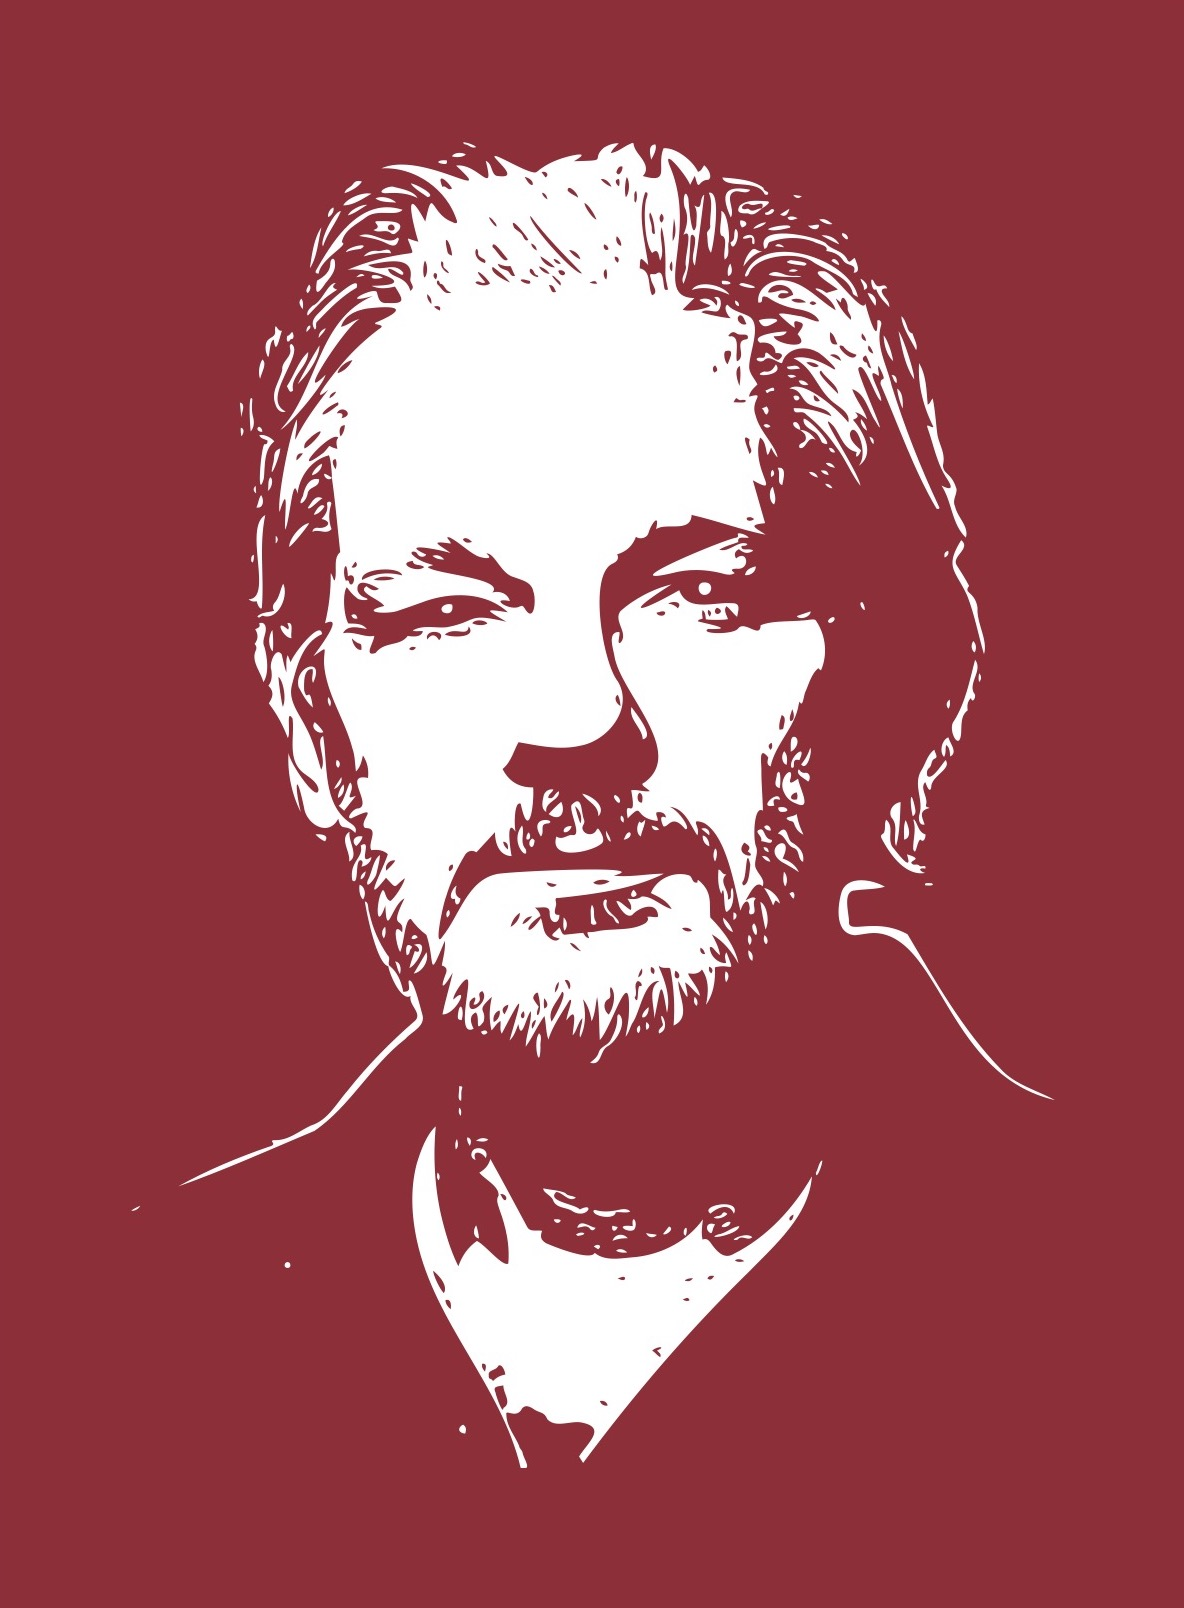
\includegraphics[width=180mm]{assange.jpg}

Herausgeber:
Martin Sonneborn
Fraktionsloses Mitglied des Europäischen Parlaments
Rue Wiertz 60
1047 Brüssel
Belgien
2. Auflage, aktualisiert. Jetzt noch deprimierender. Smiley!
Die zum Ausdruck gebrachten Meinungen liegen in der alleinigen Verantwortung der jeweiligen Verfasser
und geben nicht unbedingt den offiziellen Standpunkt des Europäischen Parlaments wieder.

\end{document}